\chapter{ادبیات موضوع و کارهای پیشین}
\clearpage

در این فصل ابتدا به معرفی و بررسی مسئله‌ی شناسایی فعالیت‌های انسانی و پژوهش‌های انجام‌شده در این زمینه می‌پردازیم. در ادامه، به بررسی روش‌های یادگیری خودنظارتی، کاربرد آن‌ها در حوزه‌ی شناسایی فعالیت انسان، و پژوهش‌های مرتبط در این زمینه خواهیم پرداخت.

شناسایی فعالیت‌های انسانی یکی از مسائل مهم و پرکاربرد در حوزه‌های مختلف از جمله سلامت، خانه‌های هوشمند و پایش رفتار کاربران به‌شمار می‌رود. همان‌گونه که در فصل مقدمه نیز بیان شد، دو رویکرد کلی برای این مسئله وجود دارد: رویکرد مبتنی بر داده‌های تصویری و رویکرد مبتنی بر داده‌های حسگری. در این پژوهش، تمرکز اصلی بر استفاده از داده‌های حسگرها بوده و از این رو، روش‌های انتخاب‌شده نیز بر پایه‌ی این نوع داده‌ها طراحی و ارزیابی شده‌اند.

\section{شناسایی فعالیت انسان}

پیشرفت‌های مختلف در تکنولوژی، باعث شده‌اند که حسگرها با هزینه‌ی اندک تولید شوند و داده‌های تولید شده توسط آن‌ها با سرعت بالا پردازش شوند که در نتیجه‌ی آن کار با حسگرها در عمل ساده می‌شود و باعث تحقیقات متعددی در این حوزه شده است. علاوه بر آن، سیستم‌های هوشمند برای عملکرد مناسب نیازمند این هستند که فعالیت انجام شده توسط کاربر شناسایی شود تا سیستم بتواند به‌خوبی کار خود را انجام دهد. در ادامه چند مورد از کاربردهای کلی شناسایی فعالیت انسان در دنیای واقعی را شرح می‌دهیم:

\begin{itemize}
\item{سیستم‌های مراقبتی}

در بیشتر سیستم‌های سنتی مراقبتی، بیماران و افراد تحت مراقبت بایستی ارزیابی‌های دوره‌ای را انجام دهند که این موضوع علاوه بر زمان‌بر و هزینه‌بر بودن، دقیق نیست. چرا که این ارزیابی‌های دوره‌ای تنها وضعیت بیمار در لحظه را مورد سنجش قرار می‌دهند و ممکن است در یک زمانی بیمار مراجعه کند که علائم به خوبی دیده نشوند. به دلایل ذکر شده، سیستم‌های مراقبتی و پزشکی استقبال گسترده‌ای از روش‌های شناسایی فعالیت مبتنی بر انواع حسگرها کرده‌اند و تلاش‌ها در راستای هوشمندسازی هر چه بیشتر سیستم‌های مراقبتی ادامه دارد.

\item{دستیار زندگی در خانه‌های هوشمند}

از سیستم‌های شناسایی فعالیت می‌توان برای مراقبت از بیماران یا سالمندان در منزل و همچنین به‌عنوان دستیار زندگی بهره گرفت. برای مثال، سامانه‌ای هوشمند برای شناسایی فعالیت توسط الاقباری و همکاران طراحی شده که علاوه بر شناسایی فعالیت‌های روزمره، قابلیت تشخیص ناهنجاری‌ها\LTRfootnote{Anomaly} (مانند زمین خوردن فرد یا هر گونه اختلال در داده‌های حسگرها) و پیش‌بینی فعالیت بعدی (مثلاً پیش‌بینی ورود فرد به اتاق خواب و فعال‌سازی سیستم تهویه) را نیز دارد. چنین سیستمی می‌تواند به‌عنوان یک دستیار زندگی در خانه‌های هوشمند عملکرد مؤثری از خود نشان دهد \cite{alaghbari2022activities}.
‪
\end{itemize}

\subsection{تعریف مسئله}

برای مسئله‌ی شناسایی فعالیت انسان دو تعریف کلی می‌توان ارائه داد.

\noindent\textbf{تعریف اول:}


فرض کنید مجموعه‌ای به صورت \( S = \{s_0, s_1, \ldots, s_{k-1}\} \) در اختیار داریم که شامل \(k\) دنباله زمانی از اندازه‌گیری‌های مربوط به ویژگی‌های مختلف است. این داده‌ها در بازه‌ی زمانی \( I = [t_{\alpha}, t_{\omega}] \) ثبت شده‌اند. در مسئله‌ی تشخیص فعالیت، هدف این است که بازه‌ی زمانی \( I \) را به زیربازه‌هایی مانند \( I_0, I_1, \ldots, I_{r-1} \) تقسیم کنیم و برای هر زیربازه، برچسبی که بیانگر نوع فعالیت است اختصاص دهیم، به‌گونه‌ای که این برچسب‌گذاری با داده‌های \( S \) تطابق داشته باشد.

بر اساس این تعریف، زیربازه‌ها باید ناتهی و بدون هم‌پوشانی باشند و کل بازه زمانی \( I \) را پوشش دهند، یعنی \( I = \bigcup_{i=0}^{r-1} I_i \). بنابراین، فرض می‌شود که در هر لحظه تنها یک فعالیت در حال انجام است. هرچند این فرض در برخی شرایط دنیای واقعی ممکن است برقرار نباشد. برای نمونه، یک فرد ممکن است همزمان در حال آشپزی و مصرف دارو باشد. این مدل ساده، چارچوبی پایه برای طراحی سیستم‌های تشخیص فعالیت فراهم می‌کند.



\noindent\textbf{تعریف دوم:}


مجموعه‌ای از \( m \) پنجره زمانی به صورت \( W = \{w_0, w_1, \ldots, w_{m-1}\} \) را در نظر بگیرید، که هر پنجره‌ی \( w_i \) شامل توالی زمانی از مشاهدات سنسورها است. برای هر پنجره‌ی زمانی، داده‌های مربوطه با مجموعه‌ای مانند \( S_i = \{s_{i,0}, \ldots, s_{i,k-1}\} \) نمایش داده می‌شوند. همچنین فرض می‌کنیم مجموعه‌ای از برچسب‌ها تحت عنوان \( L = \{l_0, \ldots, l_{m-1}\} \) موجود است که هر عنصر آن نشان‌دهنده‌ی یک نوع فعالیت در بازه‌ی متناظر با یک پنجره‌ی زمانی می‌باشد.

در این صورت، می‌خواهیم تابعی تعریف کنیم به صورت \( f: S_i \mapsto L \) که بتواند با دریافت داده‌های هر پنجره \( S_i \)، مناسب‌ترین فعالیت از \( L \) را انتخاب کند. در واقع، این تابع تلاش می‌کند تشخیص دهد که در پنجره‌ی زمانی \( w_i \) کدام فعالیت غالب بوده است. اگرچه این شیوه به فرض غالب بودن یک فعالیت در هر پنجره استوار است، اما با در نظر گرفتن هم‌پوشانی جزئی یا نویز در داده‌ها، می‌تواند تخمینی مناسب از واقعیت ارائه دهد.

نکته‌ی مهم اینجاست که اگر دو پنجره زمانی پشت سر هم باشند، برچسب آن‌ها ممکن است مشابه باشد یا حتی در مرز پنجره‌ها، فعالیتی مشترک رخ دهد. با این حال، این روش باعث می‌شود مسئله به صورت برچسب‌گذاری دنباله‌ای از پنجره‌ها ساده‌سازی شده و امکان آموزش مدل‌های یادگیری ماشین فراهم گردد.

در مجموع، این مدل به ما اجازه می‌دهد با وجود پیچیدگی‌های ذاتی رفتارهای انسانی، از طریق تحلیل پنجره‌ای و نگاشت آن به برچسب‌ها، فرایند تشخیص فعالیت را قابل پیاده‌سازی و آموزش‌پذیر سازیم. این روش به‌ویژه در محیط‌های دارای داده‌های زیاد و پیوسته که فعالیت‌ها با یکدگیر همپوشانی دارند، بسیار کاربردی و موثر خواهد بود.

رویکرد کلی برای حل مسئله‌ی شناسایی فعالیت بدین صورت است که ابتدا نیاز به یک مجموعه داده‌ی
برچسب‌دار داریم. سپس با استفاده از این مجموعه داده‌ی برچسب‌دار، سعی می‌کنیم ویژگی‌هایی را استخراج کنیم و از آن‌ها برای آموزش مدل استفاده کنیم. بدین منظور چالش‌های متعددی بوجود می‌آیند که برای حل آن‌ها رویکردهای مختلفی توسط محققان ارائه شده‌اند که در ادامه به بررسی تعدادی از آن‌ها می‌پردازیم.

\subsection{سابقه پژوهش}

در زمینه‌ی شناسایی فعالیت‌های انسانی در کاربردهای مختلف کارهای متعددی انجام شده است. همرلا و همکاران\cite{hammerla2015pd}
حسگرهای پوشیدنی را به کفش‌های ۳۴ شخص مختلف دارای بیماری
پارکینسون\LTRfootnote{Parkinson's Disease}
متصل کردند. وظیفه‌ی این حسگرها اندازه‌گیری سرعت و شیوه راه رفتن افراد بود. سپس با استخراج ویژگی‌ها از روی مقادیر خام تولیدی توسط حسگرها و با استفاده از
ماشین بولتزمن محدود (\verb|RBM|\LTRfootnote{Restricted Boltzmann Machine}
اقدام به تشخیص بیماری پارکینسون در این افراد کردند.

یک کاربرد دیگر سیستم‌های شناسایی فعالیت که به آن اشاره کردیم، استفاده از آن برای دستیار زندگی و نظارت در خانه‌ی هوشمند می‌باشد. می‌توان از این سیستم‌ها برای مراقبت از بیماران مبتلا به
بیماری فراموشی\LTRfootnote{Alzheimer's Disease} و سالمندان استفاده کرد. محققان یک روش بر مبنای
مدل‌های پنهان مارکوف\LTRfootnote{Hidden Markov Models}
ارائه دادند که می‌تواند فعالیت‌های فرد ساکن خانه را شناسایی کند و موارد اضطراری و موارد مربوط به سلامت را گزارش دهد\cite{asghari2018activity}

به‌طور کلی، روش‌های مربوط به شناسایی فعالیت‌های انسانی به روش‌های مبتنی بر یادگیری ماشین و یادگیری عمیق روی آورده‌اند. مدل‌های یادگیری عمیق بسیاری برای برای شناسایی فعالیت پیشنهاد شده استو این مدل‌ها دقت خوبی را در آموزش با داده‌های برچسب‌دار به اندازه‌ی کافی
ارائه می‌کنند\cite{cook2013transfer}.
علاوه بر آن، روش‌های یادگیری عمیق در کاربردهای استخراج ویژگی در مسائل شناسایی فعالیت که داده‌های ورودی دارای ابعاد بالایی هستند به‌کار گرفته شده‌اند. روش‌های
داده محور\cite{chen2015deep}
و مدل محور چندوجهی\LTRfootnote{Multi-modal}\cite{ha2015multi}
دو روش کاربرد مدل عمیق در مسائل تشخیص فعالیت هستند.

یک راهکار که در گذشته به نتایج خوبی دست یافت، استفاده از روش‌های سنتی یادگیری ماشین است. روش
کا-نزدیک‌ترین همسایه (\verb|KNN|)
اگرچه یک روش ساده است،‌اما برای مثال توسط
فوستر و همکاران\cite{foerster1999detection}
برای شناسایی وضعیت بدن و جهت حرکت با استفاده از داده‌های حسگر به‌کار گرفته شد و نتایج خوبی از خود نشان داد. از دیگر روش‌های مورد استفاده نیز می‌توان
مدل‌های پنهان مارکوف\cite{asghari2018activity}،
جنگل تصادفی\LTRfootnote{Random Forest}\cite{attal2015physical}
و ماشین بردار پشتیبان (\verb|SVM|\LTRfootnote{Support Vector Machine})\cite{attal2015physical}
را نام برد که در دسته‌بدنی و شناسایی فعالیت‌های انسانی دارای عملکرد نسبتا خوبی هستند. مزیت این روش‌ها این است که بر خلاف روش‌های مبتنی بر یادگیری عمیق،‌ نیازمند تعداد داده‌ی بسیار زیادی نیستند و با تعداد داده‌ی کم می‌توانند نتایج خوبی را از خود نشان دهند\cite{chen2021deep}.
اما مشکلی که این روش‌ها دارند این است که نیازمند متخصص برای
استخراج ویژگی دستی\LTRfootnote{Handcrafted Features}
هستند و علاوه بر نیاز به متخصص، ویژگی‌های استخراج شده به اندازه‌ی کافی
انتزاعی\LTRfootnote{Abstract}
و پرکاربرد نیستند. بنابراین نمی‌توان به این روش‌ها در دنیای امروز که توزیع و ابعاد داده‌ها از پیچیدگی بالایی برخوردار هستند اکتفا کرد.

با پیشرفت شبکه‌های عصبی و فراهم شدن حجم زیاد داده‌ی برچسب‌دار و همه‌گیر شدن روش‌های مبتنی بر یادگیری عمیق، در سال‌های اخیر روش‌های شناسایی فعالیت نیز به استفاده از شبکه‌های عصبی روی آورده‌اند. چرا که داده‌ها در حوزه‌ی شناسایی فعالیت‌های انسانی عموما پیچیده و دارای ابعاد بالا و در برخی موارد چند وجهی هستند. محققان نشان دادند که با در نظر گرفتن داده‌ها بصورت چندوجهی و ترکیب داده‌های انواع مختلفی از حسگرها،‌به نتایج بهتری نسبت به حالتی که تنها از یک حسگر (مانند یک شتاب‌سنج) استفاده شده است می‌توان دست یافت\cite{guo2016wearable}.
علاوه بر آن، شبکه‌های عصبی عمیق به‌دلیل ساختار چند لایه و پیچیده‌ای که دارند، هر لایه می‌تواند ویژگی‌های مختلفی را از داده استخراج کند و نتیجتا امکان کار با داده‌های پیچیده‌تر را برایمان فراهم می‌کنند. برای استخراج ویژگی توسط شبکه‌های عصبی دیگر نیاز چندانی به مهندسی ویژگی به‌صورت پیچیده و کاملا دستی نخواهیم داشت و با ساختارهای خاصی می‌توان ویژگی‌ها را به‌صورت کاملا خودکار استخراج کرد\cite{kumar2024human}. برای مثال، از شبکه‌های پیچشی یک بعدی و دو بعدی می‌توان در استخراج ویژگی‌ها و
وابستگی‌های مکانی\LTRfootnote{Spatial Dependencies}
(مثلا در تصاویر)
و همینطور از شبکه‌های بازگشتی\LTRfootnote{Recurrent Neural Network}
مانند حافظه‌ی کوتاه‌مدت بلند (\verb|LSTM|\LTRfootnote{Long Short-Term Memory})
یا واحد بازگشتی دروازه‌ای (\verb|GRU|\LTRfootnote{Gate Recurrent Unit})
در استخراج ویژگی‌ها و وابستگی‌های زمانی\LTRfootnote{Temporal Dependencies} استفاده کرد.

الاقباری و همکاران\cite{alaghbari2022activities}
در مقاله‌ی خود ۳ روش مختلف برای شناسایی فعالیت، شناسایی ناهنجاری و پیش‌بینی فعالیت ارائه دادند. آن‌ها برای هر فعالیت، یک مجموعه از \verb|R| ویژگی را تعریف می‌کنند که این ویژگی‌ها شامل موارد زیر می‌باشند:
\begin{enumerate}
    \item زمانی که برای انجام شدن فعالیت سپری شده است.
    \item تعداد حسگرهایی که در طول انجام فعالیت فعال بوده اند.
    \item تعداد دفعاتی که این فعالیت در طول روز انجام شده است.
    \item وضعیت (روشن/خاموش) تمام حسگرها
\end{enumerate}

با استفاده از تمامی این ویژگی‌ها مسئله به جای تحلیل سری به یک مسئله‌ی ساده‌تر تبدیل می‌شود که توسط
یک پرسپترون چند لایه (\verb|MLP|\LTRfootnote{Multi-Layer Perceptron})
عملیات دسته‌بندی و شناسایی فعالیت انجام می‌شود. در همین حین که شبکه‌ی پرسپترون چند لایه مشغول شناسایی فعالیت است، یک
شبکه‌ی خودکدگذار بیش‌کامل (\verb|OCDAE|\LTRfootnote{Over-Complete Deep Auto-Encoder})
وظیفه‌ی شناسایی ناهنجاری را دارد. بدین صورت که  همان \verb|R| ویژگی به این شبکه نیز داده می‌شوند و این شبکه سعی می‌کند که خروجی را از روی ورودی بازسازی کند. اگر که
خطای بازسازی\LTRfootnote{Reconstruction Error}
کم بود، بدین معناست که فعالیت مربوطه مانند یکی از فعالیت‌هایی است که شبکه قبلا بر روی آن آموزش دیده و در غیر اینصورت یک ناهنجاری شناسایی می‌شود.
\begin{figure}[htbp]
  \centering
  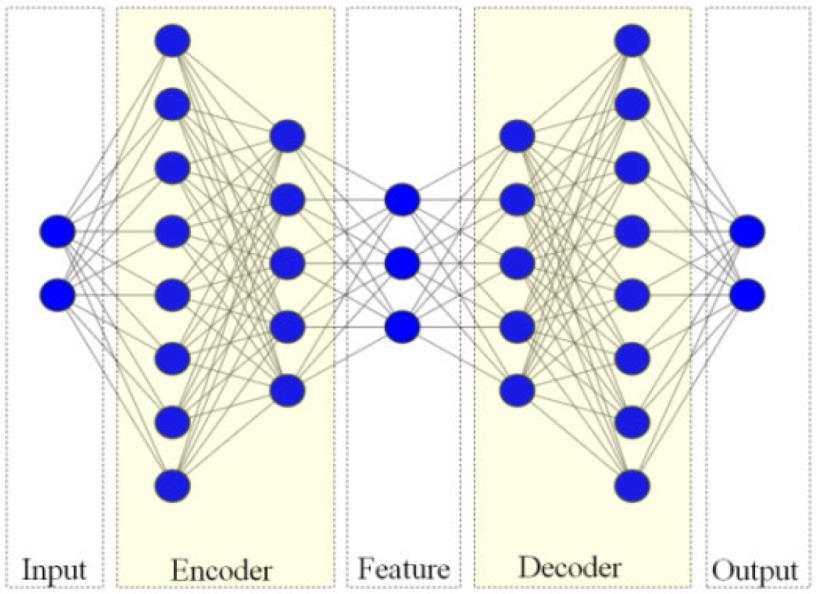
\includegraphics[width=0.8\textwidth]{Images/Chapter2/ocd-ae.png}
  \caption{ساختار خودکدگذار عمیق بیش‌کامل}
  \label{fig:ocd-ae}
\end{figure}
در عین حال که این ۲ شبکه کار می‌کنند، اگر که ناهنجاری شناسایی نشود خروجی شبکه‌ی شناسایی کننده‌ی فعالیت به‌عنوان فعالیت فعلی در نظر گرفته می‌شود و سپس توسط یک شبکه‌ی حافظه‌ی کوتاه‌مدت بلند، فعالیت بعدی پیش‌بینی می‌شود. شکل کلی ساختار پیاده شده در این مقاله به فرم شکل \ref{fig:alaghbari-framework} می‌باشد.
\begin{figure}[htbp]
  \centering
  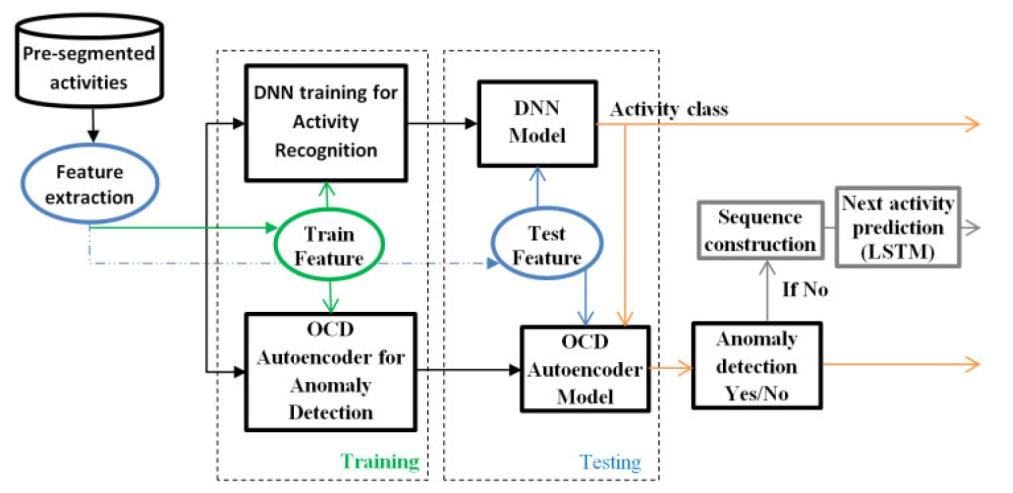
\includegraphics[width=0.8\textwidth]{Images/Chapter2/alaghbari-framework.png}
  \caption{معماری سیستم تشخیص فعالیت، ناهنجاری و پیش‌بینی فعالیت بعدی}
  \label{fig:alaghbari-framework}
\end{figure}

گائو و همکاران\cite{gao2021danhar}
یک روش بر مبنای سازوکار توجه\LTRfootnote{Attention Mechanism}
و توجه دوگانه\LTRfootnote{Dual Attention}
ارائه دادند. سازوکار توجه به شبکه‌ی عصبی این امکان را می‌دهد که به مرور یاد بگیرد که به کدام بخش‌های داده توجه بیشتری نشان دهد. برای مثال سازوکار توجه در داده‌ی تصویری به شبکه این امکان را می‌دهد که به بخش‌های مهم‌تر تصویر اهمیت بیشتری نشان بدهد و شبکه بتواند ویژگی‌های مهم‌تری را استخراج کند. توجه دوگانه بدین صورت عمل می‌کند که سازوکار توجه به‌طور همزمان برای دو نوع داده (مثلا تصویر و داده‌ی دنباله‌ای مانند متن) به‌کار گرفته شود.

بدین ترتیب گائو و همکاران از توجه دوگانه برای مسئله‌ی شناسایی فعالیت انسان استفاده کردند. روش ارائه شده چند بخش اصلی دارد:
\begin{enumerate}
    \item \textbf{ورودی داده‌های سنسورها:}
    سیگنال‌های چند-کاناله‌ی حسگرها (مانند شتاب‌سنج و ژیروسکوپ) به عنوان ورودی به مدل داده می‌شوند.

    \item \textbf{استخراج ویژگی با شبکه‌های پیچشی:}
    با عبور داده‌ها از چندین لایه شبکه‌ی پیچشی، ویژگی‌های سطح پایین و میانی استخراج می‌شوند.

    \item \textbf{ماژول توجه دوگانه:}
    پس از استخراج ویژگی، ویژگی‌های به‌دست‌آمده به ماژول توجه دوگانه داده می‌شوند. این ماژول شامل:
    \begin{itemize}
        \item \textbf{توجه کانالی\LTRfootnote{Channel Attention}:} محاسبه‌ی وزن برای هر کانال از ویژگی‌ها به‌منظور تعیین اهمیت سنسورها و ویژگی‌های مختلف و تقویت ویژگی‌های مهم.
        \item \textbf{توجه زمانی\LTRfootnote{Temporal Attention}:} محاسبه‌ی وزن برای هر گام زمانی به‌منظور تمرکز روی بازه‌های زمانی مهم در طول فعالیت.
    \end{itemize}
    ویژگی‌های خروجی از این دو توجه به‌ترتیب روی ویژگی‌ها ضرب می‌شوند و بازنمایی غنی‌شده‌ای از داده تولید می‌شود.

    \item \textbf{تکرار فرایند استخراج ویژگی و توجه:}
    فرایند استخراج ویژگی و ماژول توجه دوگانه یک بار دیگر تکرار می‌شود تا ویژگی‌های سطح بالاتری استخراج شوند.

    \item \textbf{لایه‌های دسته‌بندی:}
    در نهایت، ویژگی‌های استخراج و وزن‌دهی شده به لایه‌های تماما متصل\LTRfootnote{Fully Connected} داده می‌شوند تا فعالیت مربوطه پیش‌بینی شود.
\end{enumerate}
\begin{figure}[htbp]
  \centering
  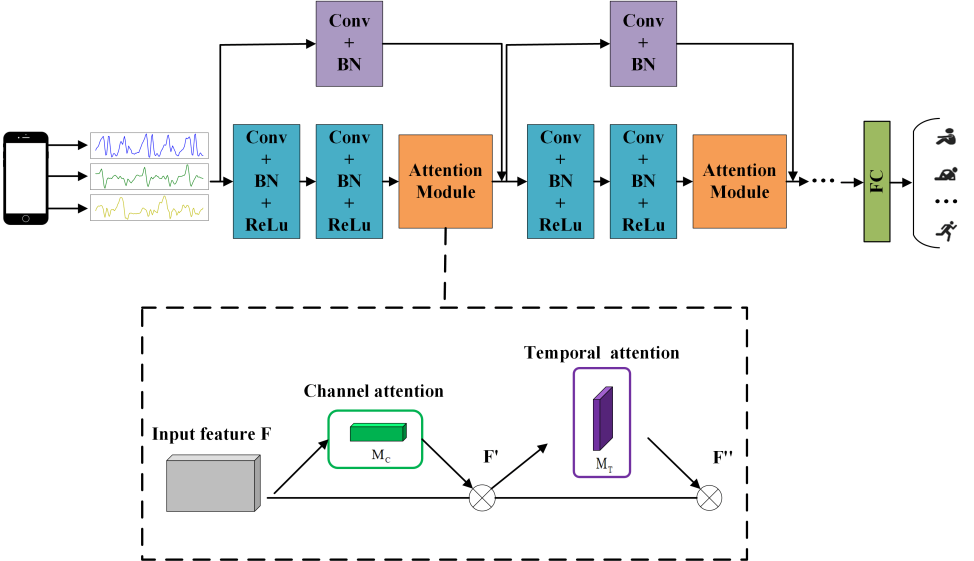
\includegraphics[width=0.8\textwidth]{Images/Chapter2/danhar.png}
  \caption{معماری سیستم توجه دوگانه بر روی داده‌های حسگر}
  \label{fig:danhar}
\end{figure}

وانگ و همکاران\cite{wang2020wearable} یک روش مبتنی بر ترکیب شبکه پیچشی و شبکه حافظه کوتاه‌مدت بلند ارائه کردند که به دقت بالایی دست یافت. در این روش، از داده‌های مربوط به سری زمانی دو حسگر ۳ کاناله شتاب‌سنج و ژیروسکوپ ابتدا
پنجره‌های لغزان\LTRfootnote{Sliding Windows}
دارای همپوشانی استخراج می‌شوند و سپس داده‌های هر ۶ کانال حسگرها به صورت یک تصویر در کنار هم قرار می‌گیرند. بدین صورت یک تصویر به طول پنجره‌ی لغزان و عرض ۶ خواهیم داشت. سپس بر روی این شبه تصاویر لایه‌های پیچشی اعمال می‌شوند و آرایه‌ای از این شبه تصاویر توسط لایه‌های پیچشی پردازش می‌شوند تا ویژگی‌های هر پنجره که با دیگر پنجره‌ها همپوشانی دارد استخراج شوند. سپس این دنباله ویژگی‌های استخراج شده به یک شبکه حافظه کوتاه‌مدت بلند داده می‌شود که خروجی آن مجموعه‌ای از بردارها است که شامل وابستگی‌های زمانی و توالی فعالیت‌ها می‌باشد. این بردارها به لایه‌ی تماما متصل داده می‌شوند تا ویژگی‌های کلی فعالیت با یکدیگر
ترکیب\LTRfootnote{Fusion}
شده و به‌صورت یکپارچه استخراج شوند. ضمنا جهت پایداری بیشتر یادگیری و دستیابی به دقت بالاتر، نویسندگان مقاله از
نرمال‌سازی دسته‌ای\LTRfootnote{Batch Normalization}
استفاده کردند.

لیو و همکاران\cite{liu2025set} در مقاله‌ی خود با عنوان
«\lr{SETransformer}»
یک معماری ترکیبی مبتنی بر ترنسفورمر را برای شناسایی فعالیت‌های انسانی معرفی کردند. این مدل از سه مؤلفه اصلی تشکیل شده است:

\begin{enumerate}
    \item \textbf{کدگذار مبدل برای مدل‌سازی وابستگی‌های زمانی سراسری:}
    با استفاده از لایه‌های خودتوجهی چندسر\LTRfootnote{Multi-Head Self-Attention}، این بخش قادر است وابستگی‌های بلندمدت در پنجره‌های زمانی طولانی را به خوبی مدل کند.

    \item \textbf{ماژول فشرده-وبرانگیزش\LTRfootnote{Squeeze-and-Excitation} برای توجه کانالی:}
    این ماژول به صورت پویا اهمیت هر یک از کانال‌های حسگر (مانند محورهای \lr{x}، \lr{y} و \lr{z} شتاب‌سنج) را با توجه به زمینه کلی فعالیت، بازتنظیم می‌کند.

    \item \textbf{مکانیزم توجه زمانی برای تجمیع بازنمایی‌های زمانی:}
    به جای استفاده از روش‌های ثابت مانند میانگین‌گیری سراسری، این مکانیزم به مدل اجازه می‌دهد تا گام‌های زمانی مهم را برای دسته‌بندی نهایی، انتخاب و تقویت کند.
\end{enumerate}

مدل پیشنهادی آن‌ها بر روی مجموعه‌داده \lr{WISDM} ارزیابی شده و نتایج نشان می‌دهد که این روش از نظر دقت، عملکرد بهتری نسبت به مدل‌های مرسوم مانند \lr{LSTM}، \lr{GRU}، \lr{BiLSTM} و \lr{CNN} دارد. این معماری به دلیل قابلیت تفسیرپذیری و تمرکز انتخابی بر بخش‌های کلیدی سیگنال، گامی به سوی شناسایی فعالیت‌های انسانی قوی و قابل اعتماد در محیط‌های واقعی محسوب می‌شود.

لی و همکاران\cite{li2023human} یک چارچوب کامل برای شناسایی فعالیت‌های روزمره در محیط‌های هوشمند چندساکنه ارائه کردند. روش پیشنهادی آن‌ها با نام \lr{HAR\_WCNN} شامل سه مرحله‌ی اصلی است:
\begin{enumerate}
\item \textbf{انتخاب حسگر مبتنی بر تحلیل اهمیت (\lr{CSA}):} با الهام از مفاهیم \lr{TF-IDF} و تئوری اطلاعات، روشی برای سنجش میزان مشارکت هر نوع حسگر در شناسایی هر فعالیت ارائه شد. این امر به انتخاب خودکار حسگرهای مؤثر و کاهش حجم داده‌های پردازشی کمک می‌کند.
\item \textbf{پیش‌پردازش داده با ماتریس فاصله‌ی فضایی (\lr{SDM}):} برای کاهش نویز ناشی از فعالیت‌های متقاطع چندین ساکن، یک ماتریس فاصله بر اساس چیدمان حسگرها در خانه ساخته شد تا داده‌های نامرتبط حذف شوند.
\item \textbf{دسته‌بندی با شبکه‌ی عصبی کانولوشنی بازه‌ی زمانی گسترده (\lr{WCNN}):} یک شبکه‌ی \lr{CNN} یک‌بعدی با هسته‌های کانولوشن بزرگ طراحی شد تا وابستگی‌های بلندمدت در داده‌های سری‌زمانی به‌خوبی می‌شود. این معماری سبک‌وزن، در مقایسه با \lr{LSTM}، سرعت پردازش بسیار بالاتری دارد.
\end{enumerate}

نتایج آزمایش‌ها روی مجموعه‌داده‌ی \lr{CASAS} نشان داد که \lr{HAR\_WCNN} هم از نظر دقت شناسایی و هم از نظر سرعت، عملکرد بهتری نسبت به روش‌های پایه دارد. این رویکرد به‌ویژه برای محیط‌های واقعی با داده‌های پرنویز و چندساکنه مناسب است.

لی و همکاران \cite{li2024sensorllm} در مقاله‌ی «\lr{SensorLLM}» چارچوبی نوین برای یکپارچه‌سازی داده‌های حسگر حرکت با مدل‌های زبانی بزرگ (\lr{LLM}) جهت شناسایی فعالیت انسان ارائه کردند. این چارچوب دو مرحله‌ای، ابتدا در مرحله \lr{Sensor-Language Alignment}، داده‌های سری‌زمانی حسگر را با توصیف‌های متنی مبتنی بر روند (\lr{Trend}) هم‌تراز می‌سازد. این هم‌ترازی با تولید خودکار جفت‌های پرسش و پاسخ از طریق تحلیل‌های آماری و قالب‌های ازپیشتعیین‌شده و بدون نیاز به حاشیه‌نویسی دستی انجام می‌شود. برای این کار از یک کدگذار سری‌زمانی (\lr{Chronos}) و یک لایه \lr{MLP} برای نگاشت بازنمایی‌های حسگر به فضای درک‌شده توسط \lr{LLM} استفاده می‌شود. همچنین با معرفی توکن‌های ویژه برای مرزبندی کانال‌های مختلف حسگر، وابستگی‌های بین کانالی حفظ می‌شود. در مرحله دوم، یعنی \lr{Task-Aware Tuning}، از بازنمایی‌های هم‌تراز شده برای آموزش یک مدل دسته‌بندی سبک بر روی \lr{LLM} (با پارامترهای ثابت) برای انجام وظیفه شناسایی فعالیت استفاده می‌گردد. نتایج تجربی بر روی پنج مجموعه‌داده نشان می‌دهد که این روش نه تنها در درک روند داده‌های حسگر از \lr{GPT-4o} پیشی می‌گیرد، بلکه در کار دسته‌بندی نیز با مدل‌های مطرح رقابت می‌کند یا از آن‌ها فراتر می‌رود. این کار پایه‌ای برای توسعه مدل‌های بنیادین چندوجهی برای تحلیل داده‌های حسگر می‌گذارد.

\section{یادگیری خودنظارتی}

همانطور که در بخش قبل بررسی کردیم، شبکه‌های عصبی عمیق در مواردی که داده‌ها از پیچیدگی بالایی برخوردار هستند و ابعاد داده‌های ورودی بالا هستند، شدیدا از روش‌های سنتی یادگیری ماشین عملکرد بهتر و قدرتمندتری دارند و نتایج دقیق‌تری را از خود نشان می‌دهند. در واقع می‌توان گفت که در کاربردهای پیشرفته‌ی دنیای امروز استفاده از یادگیری عمیق به روش‌های یادگیری ماشین سنتی در اکثر مواقع ترجیح داده می‌شوند. اما چالش اصلی روش‌های مبتنی بر یادگیری عمیق نیاز شدید این روش‌ها به حجم زیادی داده برچسب‌گذاری شده می‌باشد. آنچه که در دنیای امروز شدیدا فراوان و در دسترس است، انواع داده بدون برچسب می‌باشد و به‌طور کلی جمع‌آوری داده‌ی خام کاری نسبتا ساده و کم‌هزینه می‌باشد. اما برچسب‌گذاری داده‌ها کاری شدیدا پرهزینه و زمان‌بر می‌باشد. در واقع یکی از اصلی‌ترین
گلوگاه‌های\LTRfootnote{Bottleneck}
آموزش شبکه‌های عصبی عمیق، جمع‌آوری داده‌ی آموزشی دارای برچسب می‌باشد.

علاوه بر هزینه‌ها و چالش‌های ناشی از برچسب‌گذاری داده‌ها، یادگیری تحت نظارت دارای مشکلاتی مانند 
خطای تعمیم\LTRfootnote{Generalization Error}،
همبستگی‌های کاذب\LTRfootnote{Spurious Correlations}
و برچسب‌گذاری‌های غلط غیر عمدی و یا عمدی ناشی از حملات خصمانه\LTRfootnote{Adversarial Attacks}
می‌باشد\cite{liu2021self}.

با توجه به تمامی چالش‌های ذکر شده، ضروری است که به سراغ روش‌هایی برویم که وابستگی ما را به مجموعه داده‌های برچسب‌دار کاهش دهند. هدف اصلی، دستیابی به قابلیت اجرای مانند دسته‌بندی تنها با اتکا به حجم به مراتب کمتری از داده‌های برچسب‌خورده است.

برای تحقق این هدف، رویکردهایی مانند یادگیری خودنظارتی بسیار کارآمد هستند. روش‌های مبتنی بر یادگیری خودنظارتی به ما اجازه می‌دهند تا از ظرفیت عظیم داده‌های بدون برجسب که به وفور یافت می‌وشند و دسترسی به آن‌ها کم‌هزینه‌تر است بهره ببریم. در این شیوه، مدل ابتدا با استفاده از داده‌های خام و بدون برچسب، یک درک پایه‌ای و غنی از ساختار و ویژگی‌های داده‌ها پیدا می‌کند. سپس این مدل پیش‌آموخته را می‌توان با مقدار بسیار اندکی از داده‌های برچسب‌دار برای عملیات نهایی مورد نظر تنظیم دقیق کنیم. این رویکرد نه تنها باعث صرفه‌جویی چشمگیری در هزینه و زمان برچسب‌زنی می‌شود، بلکه به مدل اجازه می‌دهد تا با یادگیری از گستره وسیع‌تری از داده‌ها، به تعمیم‌پذیری و عملکرد بهتری دست یابد.

\begin{figure}[htbp]
  \centering
  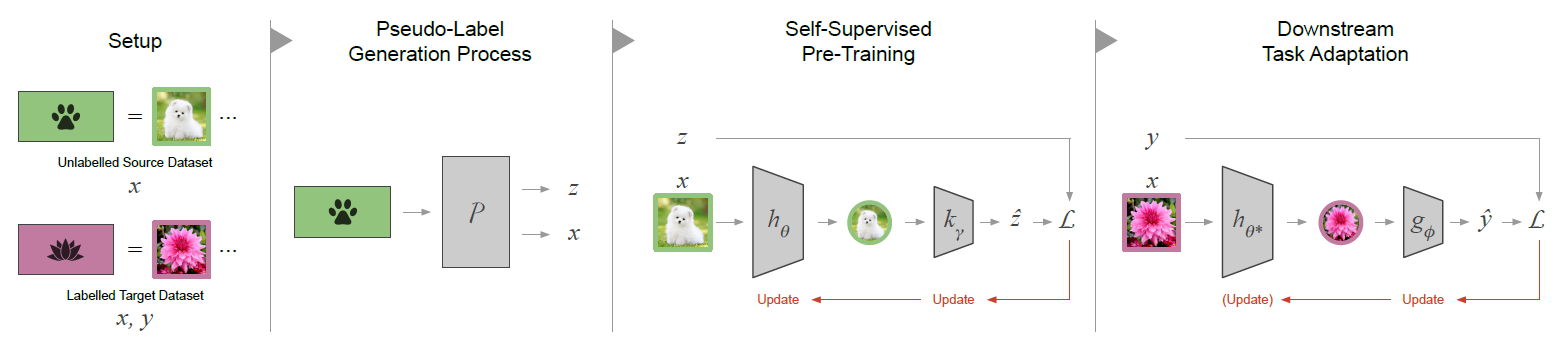
\includegraphics[width=1.0\textwidth]{Images/Chapter2/selfsupervised-overview.png}
  \caption{ساختار کلی سیستم‌های یادگیری خودنظارتی}
  \label{fig:selfsupervised-overview}
\end{figure}

\subsection{تعریف یادگیری خودنظارتی}

پیش از ارائه‌ی یک تعریف برای یادگیری خودنظارتی، برای درک بهتر مفاهیم بکار گرفته شده در این پایان‌نامه به بیان برخی از اصطلاحات که در این حوزه رایج هستند می‌پردازیم:

\begin{itemize}
    \item \textbf{شبه برچسب:}
    در حقیقت، شبه‌برچسب‌ها برچسب‌هایی هستند که معمولا به‌صورت خودکار و بر اساس ویژگی‌های داده‌ها در فاز اول آموزش (پیش‌آموزش) برای هر داده تولید می‌شوند. برای مثال در وظیفه‌ی پوششی شناسایی میزان چرخش تصویر، شبه برچسب مربوطه میزان چرخش اعمال شده به این تصویر می‌باشد.
    \item \textbf{وظیفه پوششی:}
    وظیفه پوششی در واقع وظیفه‌ای است که برای اجرای فاز پیش‌آموزش خودنظارتی طراحی شده و هدف آن یادگیری ویژگی‌های سطح بالا از روی داده‌های خام با کمک شبه‌برچسب‌ها می‌باشد. این وظیفه در حقیقت معماری شبکه و نحوه یادگیری ویژگی‌ها در فاز پیش‌آموزش خودنظارتی را تعیین می‌کند.
    \item \textbf{وظیفه پایین‌دستی\LTRfootnote{Downstream Task}:}
    وظیفه پایین‌دستی در واقع همان وظیفه اصلی است که پس از فاز پیش‌آموزش خودنظارتی انجام می‌شود که به‌طور کلی به دو منظور انجام می‌شود. هدف اول، ارزیابی کیفیت ویژگی‌های استخراج شده توسط شبکه‌ی پیش‌آموزش دیده و هدف دوم، آموزش نهایی مدل برای هدف اصلی (مثلا شناسایی فعالیت انسان یا دسته‌بندی تصاویر) می‌باشد. در واقع وظیفه‌ی پایین‌دستی شامل وظایف مستقل از پیش‌آموزش خودنظارتی است که مدل پیش‌آموزش دیده شده را به‌صورت کاربردی مورد ارزیابی قرار می‌دهد و آن را برای کاربردهای دنیای واقعی آماده می‌کند.
\end{itemize}

یادگیری خودنظارتی، یک رویکرد یادگیری ماشین است که در آن مدل بدون استفاده از برچسب‌های داده‌ها و مجموعه داده‌ی برچسب‌دار، از داده‌های بدون برچسب برای یادگیری بازنمایی‌های مفید استفاده می‌کند. در این روش، با ایجاد شبه برچسب‌ها از داده‌های ورودی بدون برچسب (مثلا حذف بخشی از داده و تلاش برای بازسازی آن) یک وظیفه پوششی تعریف می‌کنیم تا مدل بتواند ساختارها و الگوهای درونی داده را یاد بگیرد. سپس این بازنمایی‌های آموخته شده می‌توانند برای حل وظایف پایین‌دستی اصلی مانند دسته‌بندی مورد استفاده قرار بگیرند. نکته‌ی حائز اهمیت در اینجا این است که با تعداد بسیار کمتری داده‌ی برچسب‌دار می‌توان آموزش مدل را انجام داد و به قدرت تعمیم بالایی دست یافت.

\begin{figure}[htbp]
  \centering
  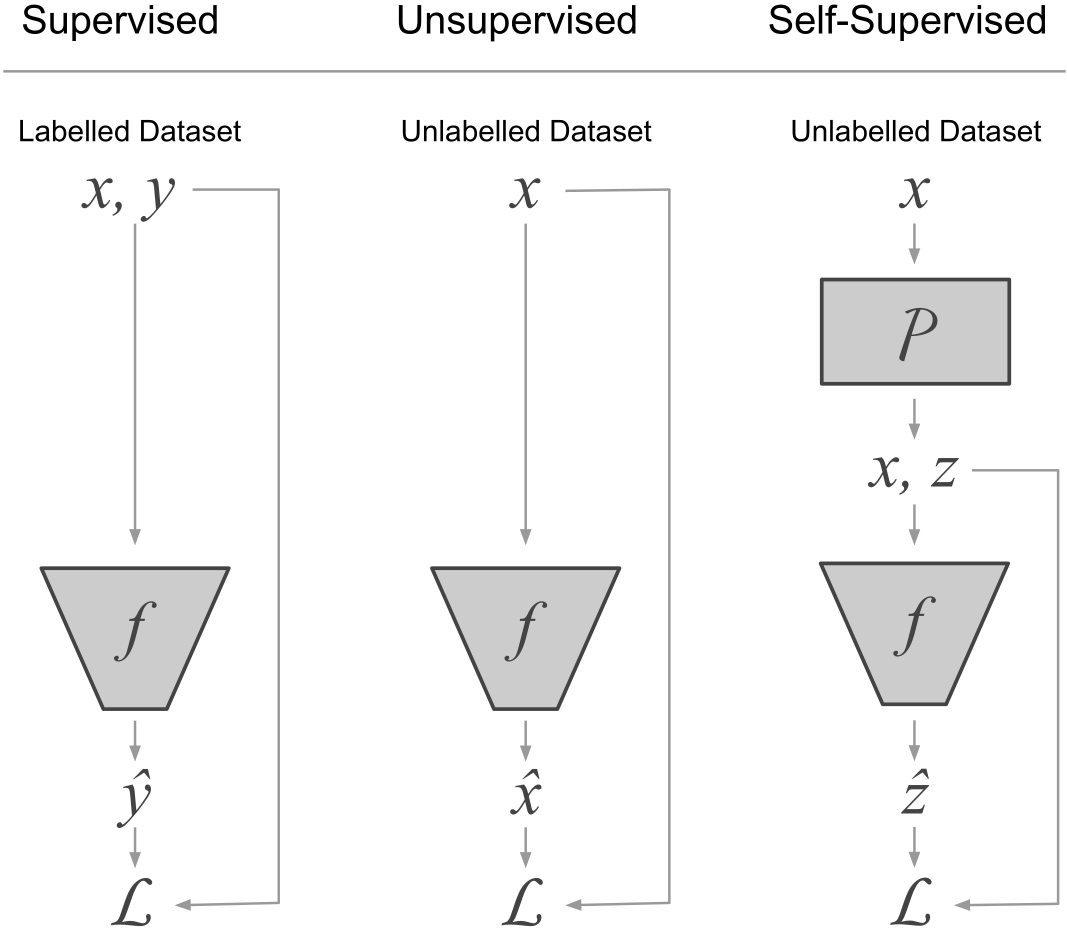
\includegraphics[width=0.7\textwidth]{Images/Chapter2/self-vs-unsupervised.png}
  \caption{ساختار کلی سیستم‌های یادگیری خودنظارتی}
  \label{fig:self-vs-unsupervised}
\end{figure}

همانطور که در شکل \ref{fig:self-vs-unsupervised}
دیده می‌شود، یادگیری خودنظارتی در اصل نوعی از یادگیری بدون نظارت است\cite{ericsson2022self}.
یادگیری بدون نظارت شامل الگوریتم‌هایی مانند انواع
الگوریتم‌های خوشه‌بندی\LTRfootnote{Clustering}،
شبکه‌ی مولد تخاصمی (\verb|GAN|\LTRfootnote{Generative Adversarial Network})
و خودکدگذار متغیر (\verb|VAE|\LTRfootnote{Variation Auto-Encoder})
می‌باشد. یادگیری خودنظارتی نیز در این موضوع که مجموعه داده بدون برچسب می‌باشد با یادگیری بدون نظارت مشترک است. اما معماری کلی و
بهینه‌سازی\LTRfootnote{Optimization}
مدل‌های یادگیری خودنظارتی به روش‌های یادگیری نظارت‌شده نزدیک‌تر است. چرا که سیگنال نظارت را توسط شبه برچسب‌ها و وظایف پوششی اعمال می‌کنیم و با شبه برچسب‌ها می‌توان دقیقا مانند یک برچسب واقعی رفتار کنیم و عمل دسته‌بندی و بهینه‌سازی مدل را با محاسبه‌ی خطای دسته‌بندی انجام دهیم.

\subsubsection{فرمول‌بندی یادگیری خودنظارتی}

در یادگیری خودنظارتی، برخلاف یادگیری با نظارت که به داده‌های جفت‌شده‌ی $X_i$ و $Y_i$ نیاز دارد (که $Y_i$ توسط نیروی انسانی برچسب‌گذاری می‌شود)، از برچسب‌هایی استفاده می‌شود که به صورت خودکار و بدون نیاز به مداخله‌ی انسانی تولید می‌شوند. این برچسب‌های خودکار یا شبه‌برچسب‌ها ($P_i$) مستقیماً از ویژگی‌های درونی داده‌ها (مانند تصاویر یا داده‌های سری‌زمانی) و با استفاده از قواعد و طراحی الگوریتمی مناسب استخراج می‌گردند. بنابراین با داشتن $N$ نمونه داده‌ی آموزشی، تابع هزینه در یادگیری با نظارت طبق رابطه‌ی زیر محاسبه می‌شود \cite{jing2020self}:

\begin{equation}
\label{eq:1-2}
loss(D) = \min_{\theta} \frac{1}{N} \sum_{i=1}^{N} loss(f_θ(X_i), Y_i)
\end{equation}

اما در فاز نخست یادگیری خودنظارتی که با هدف یادگیری بازنمایی‌های غنی از داده‌ها و استخراج ویژگی‌های باکیفیت بدون نیاز به برچسب انسانی انجام می‌شود، تابع هزینه‌ی رابطه‌ی \ref{eq:1-2} به شکل زیر تغییر پیدا می‌کند:

\begin{equation}
\label{eq:2-2}
loss(D) = \min_{\theta} \frac{1}{N} \sum_{i=1}^{N} loss(f_θ(X_i), P_i)
\end{equation}

در این معادلات، $f_θ(X_i)$ به این معنا است که ابتدا خروجی شبکه برای $X_i$ محاسبه می‌گردد و سپس مقدار آن با برچسب‌ها یا شبه برچسب‌ها مقایسه می‌شود و هزینه محاسبه می‌گردد. این فرایند باعث می‌شود که شبکه به‌تدریج پارامترهای خود را به گونه‌ای تنظیم نماید که خروجی‌های تولید شده بیشترین تطابق را با برچسب‌های موجود داشته باشند و در نتیجه مدل قادر به یادگیری الگوهای موثر و معنادار از داده‌های ورودی گردد.

پس از پایان این مرحله، مدل آموزش‌دیده در فاز پیش‌آموزش خودنظارتی آماده می‌شود تا در مرحله‌ی بعدی، یعنی آموزش با نظارت در وظایف پایین‌دستی مورد استفاده قرار گیرد. در این مرحله، از بازنمایی‌های یادگرفته‌شده توسط مدل برای بهبود کارایی و کاهش نیاز به داده‌های برچسب‌خورده‌ی فراوان استفاده می‌شود و فرایند یادگیری انتقالی به اجرا درمی‌آید.

\subsection{سابقه پژوهش}

به‌طور کلی کارهای انجام شده در حوزه‌ی یادگیری خودنظارتی را می‌توان بر حسب ماهیت وظیفه‌ی پوششی مورد استفاده به چند دسته‌ی کلی تقسیم‌بندی کرد:

\begin{enumerate}

\item \textbf{روش‌های زمینه‌محور\LTRfootnote{Context-based}:} \
در این دسته از روش‌ها، هدف مدل، یادگیری روابط میان اجزای مختلف داده با استفاده از زمینه‌ی محلی یا سراسری آن است. این روش‌ها معمولاً بر پایه‌ی روش‌هایی مانند پیش‌بینی موقعیت نسبی بخش‌های داده، ترتیب وقوع رویدادها، یا ویژگی‌های ساختاری مانند شناسایی جهت چرخش یا ترتیب قطعات بنا می‌شوند. از آنجا که این وظایف معمولاً نیاز به بازسازی کامل داده ندارند و تنها از اطلاعات ضمنی در خود داده استفاده می‌کنند، پیاده‌سازی نسبتاً ساده‌تری دارند و در حوزه‌هایی نظیر پردازش تصویر و تحلیل سیگنال کاربرد گسترده‌ای یافته‌اند.

\item \textbf{روش‌های بازسازی‌محور\LTRfootnote{Reconstruction-based}:} \
در این روش‌ها، شبکه تلاش می‌کند تا ورودی ناقص، دارای نویز یا کدگذاری‌شده را بازسازی کند. این دسته شامل خانواده‌ی گسترده‌ای از روش‌های مولد\LTRfootnote{Generative}
نیز می‌شود، از جمله خوکدگذارها، حذف نویز، رنگی‌سازی تصاویر، و پر کردن بخش‌های حذف‌شده از داده. تمرکز اصلی این رویکردها بر حفظ اطلاعات کامل از ورودی در بازنمایی‌های آموخته‌شده است. چنین بازنمایی‌هایی معمولاً ظرفیت بالایی برای انتقال به وظایف پایین‌دستی مانند طبقه‌بندی یا تشخیص دارند.

\item \textbf{روش‌های برچسب معنایی‌محور\LTRfootnote{Semantic Label-based}:} \
در این رویکردها، هدف از وظیفه‌ی پوششی، پیش‌بینی برچسب‌هایی است که به‌صورت خودکار و بدون دخالت انسان از داده استخراج شده‌اند، اما نمایانگر مفاهیم سطح بالای معنایی هستند. برای نمونه، دسته‌بندی داده‌ها بر اساس خوشه‌بندی بازنمایی‌های اولیه یا پیش‌بینی ویژگی‌هایی که نمایانگر ساختار مفهومی داده هستند. در واقع، این روش‌ها سعی می‌کنند با اجرای الگوریتم‌هایی، یک یا چند برچسب برای داده‌ها استخراج کنند و یادگیری را با استفاده از این برچسب‌ها انجام می‌دهیم. به همین دلیل، معمولاً از مکانیزم‌هایی مانند خوشه‌بندی، خودتقطیر\LTRfootnote{Self-distillation}،
یا یادگیری مبتنی بر نماینده‌ها بهره می‌برند. در این پایان‌نامه با جزئیات به آن نمی‌پردازیم اما نمونه‌ای از کاربرد این روش را می‌توان در مقاله‌ی ارائه شده توسط دتون و همکاران\cite{detone2018superpoint}
مشاهده نمود.

\item \textbf{روش‌های تباینی:} \
این دسته از روش‌ها بر اساس اصل نزدیک‌سازی نمونه‌های مشابه و دورسازی نمونه‌های ناسازگار از یکدیگر عمل می‌کنند. در این رویکرد، نمونه‌های مثبت (مانند دو نمایش\LTRfootnote{View}
مختلف از یک داده) باید در فضای بازنمایی به یکدیگر نزدیک شوند و نمونه‌های منفی (مانند دو نمایش مختلف از دو داده‌ی مختلف) از هم فاصله بگیرند. این مکانیزم باعث می‌شود که مدل، بازنمایی‌هایی مقاوم نسبت به تغییرات بی‌اهمیت یاد بگیرد. روش‌های تباینی نقش مهمی در موفقیت یادگیری خودنظارتی مدرن داشته‌اند و پایه‌گذار بسیاری از مدل‌های پیشرفته در حوزه‌های تصویر، ویدیو و سیگنال هستند.

\end{enumerate}

در ادامه، به بررسی دقیق‌تر هریک از دسته‌های یادگیری خودنظارتی معرفی شده در بالا پرداخته و نمونه‌هایی از روش‌های برجسته در هر دسته معرفی می‌شوند.

\subsubsection{روش‌های زمینه‌محور}

در روش‌های زمینه‌محور، ایده‌ی اصلی استفاده از اطلاعات زمینه‌ای موجود در خود داده برای تعریف یک وظیفه‌ی یادگیری است. این وظایف معمولا بر پایه‌ی روابط مکانی، زمانی یا ساختاری میان اجزای مختلف یک نمونه شکل می‌گیرند. چنین روش‌هایی با بهره‌گیری از ساختار درونی داده، سعی در استخراج بازنمایی‌هایی دارند که بتوانند موقعیت، ترتیب، یا سایر روابط میان اجزا را درک کنند. این دسته از روش‌ها به‌ویژه در حوزه‌های بینایی ماشین و تحلیل سیگنال، نقطه‌ی آغاز پژوهش‌های جدی در یادگیری خودنظارتی بوده‌اند و هنوز هم کاربرد گسترده‌ای دارند.\newline\newline

\noindent\textbf{وظیفه‌ی پوششی پیش‌بینی چرخش:}

یکی از وظایف پوششی مشهور در حوزه‌ی یادگیری خودنظارتی، پیش‌بینی میزان چرخش اعمال‌شده بر تصویر است. این وظیفه که نخستین بار در مقاله‌ی \lr{RotNet} \cite{gidaris2018unsupervised} معرفی شد، بر این فرض استوار است که یک شبکه‌ی عصبی تنها در صورتی قادر به تشخیص زاویه‌ی چرخش یک تصویر خواهد بود که بتواند به درک عمیقی از ساختار درونی و مفاهیم معنایی موجود در تصویر دست یابد. از این رو، پیش‌بینی چرخش به‌عنوان یک وظیفه‌ی ساده و مشخص، در عمل منجر به یادگیری بازنمایی‌هایی می‌شود که برای بسیاری از وظایف پایین‌دستی نیز قابل انتقال هستند.

در پیاده‌سازی اولیه‌ی این ایده، تصویر ورودی به‌صورت تصادفی یکی از چهار چرخش صفر، ۹۰، ۱۸۰ یا ۲۷۰ درجه را دریافت می‌کند. مدل باید زاویه‌ی صحیح را از میان چهار گزینه تشخیص دهد. برای این منظور، ساختار مدل از چندین لایه‌ی پیچشی  برای استخراج ویژگی استفاده می‌کند و در نهایت به یک لایه‌ی کاملاً متصل با چهار نورون خروجی منتهی می‌شود که هر نورون نمایانگر یکی از کلاس‌های زاویه‌ی چرخش است. این ساختار در شکل \ref{fig:rotnet} نمایش داده شده است.

\begin{figure}[htbp]
\centering
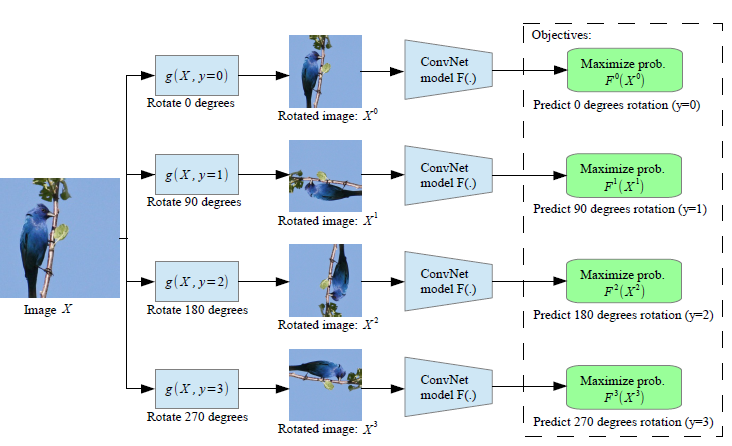
\includegraphics[width=0.8\textwidth]{Images/Chapter2/rotnet.png}
\caption{ساختار کلی شبکه‌ی پیش‌بینی چرخش}
\label{fig:rotnet}
\end{figure}

برتری اصلی این روش در آن است که بدون استفاده از هیچ‌گونه برچسب دستی، مدل را وادار می‌کند تا ساختار اشیاء، موقعیت اجزای تصویر و ویژگی‌های کلان معنایی را در بازنمایی‌های درونی خود بیاموزد. این بازنمایی‌ها در مراحل بعدی می‌توانند برای وظایفی نظیر طبقه‌بندی تصویر یا شناسایی اشیاء مورد استفاده قرار گیرند.

\begin{table}[htbp]
\centering
\caption{مقایسه‌ی عملکرد روش پیش‌بینی چرخش }
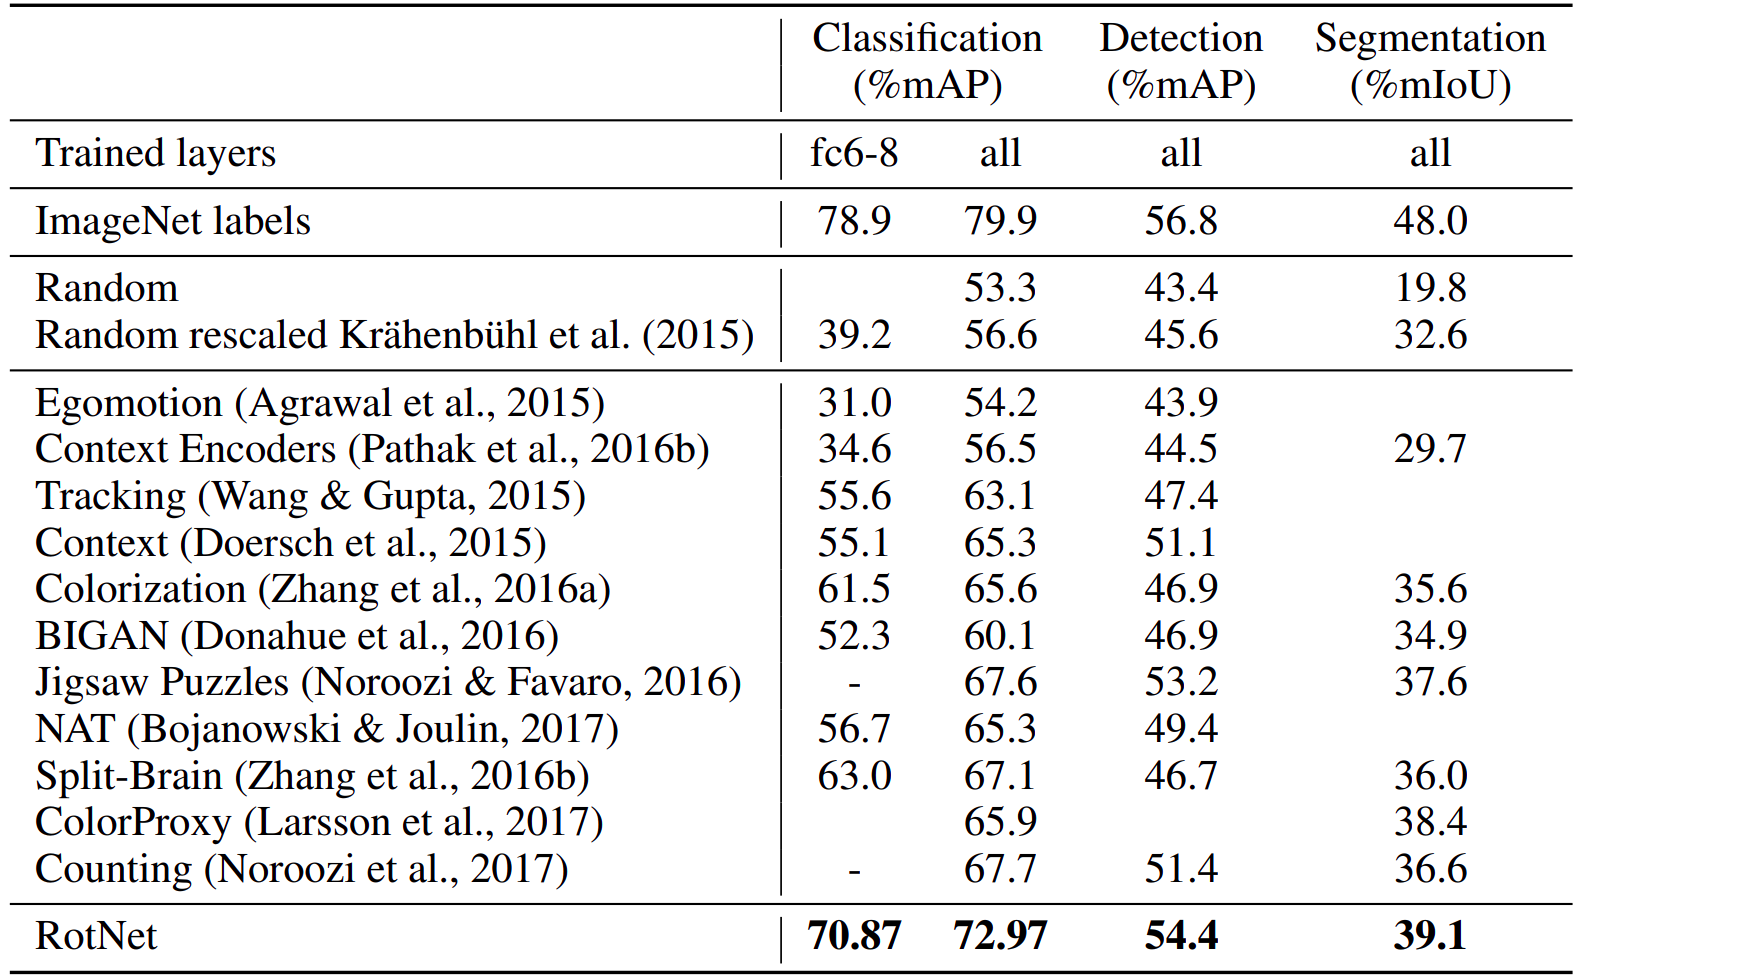
\includegraphics[width=0.8\textwidth]{Images/Chapter2/rotnet-results.png}
\label{tab:rotnet-results}
\end{table}

همان‌گونه که در جدول
\ref{tab:rotnet-results}
دیده می‌شود، عملکرد مدل پیش‌آموزش‌دیده با استفاده از وظیفه‌ی پوششی پیش‌بینی چرخش و سپس تنظیم دقیق برای انجام وظیفه‌ی پایین‌دستی اصلی، نه‌تنها از سایر روش‌های خودنظارتی و بدون نظارت موجود در زمان خود پیشی گرفته، بلکه عملکردی نزدیک به مدل‌های نظارت‌شده نیز از خود نشان داده است. این امر نشان‌دهنده‌ی قدرت وظایف ساده‌ی زمینه‌محور در هدایت مدل به سمت درک معنایی از داده‌های ورودی است.\newline

\noindent\textbf{وظیفه‌ی پوششی حل پازل\LTRfootnote{Jigsaw Puzzle}:}

یکی دیگر از روش‌های برجسته در یادگیری خودنظارتی زمینه‌محور، وظیفه‌ی حل پازل است که نخستین بار توسط نوروزی و فاوارو در مقاله‌ای تأثیرگذار ارائه شد \cite{noroozi2016unsupervised}. ایده‌ی اصلی این روش بر آن استوار است که مدل برای تشخیص نحوه‌ی قرارگیری صحیح اجزای تصویر، ناگزیر به درک دقیق ساختار داخلی تصویر، موقعیت اجزای اشیاء، و روابط مکانی بین آن‌ها خواهد بود. این درک ساختاری موجب می‌شود که مدل به بازنمایی‌هایی دست یابد که نه‌تنها ویژگی‌های محلی تصویر (مانند لبه‌ها و بافت‌ها) بلکه مفاهیم سطح بالای معنایی (مانند موقعیت اعضای یک شیء یا ارتباط بین اشیاء) را نیز منعکس کنند.

در فرایند این وظیفه‌ی پوششی، ابتدا تصویر اصلی به یک برش با ابعاد \lr{$225 \times 225$} تبدیل می‌شود. سپس این تصویر به ۹ قسمت مساوی \lr{$75 \times 75$} تقسیم شده و از هر کدام، یک برش تصادفی \lr{$64 \times 64$} استخراج می‌شود. هدف از این کار، حذف مرزهای دقیق بین قطعات و جلوگیری از وابستگی مدل به صرفِ تشخیص مرزها برای حل پازل است؛ به‌عبارت دیگر، مدل باید به جای تکیه بر نشانه‌های مصنوعی، ویژگی‌های معنایی واقعی تصویر را فرا بگیرد.

پس از آن، قطعات تصویر به صورت یک بردار ۹ تایی مسطح‌سازی شده و یکی از ۱۰۰ جایگشت از پیش تعیین‌شده روی آن اعمال می‌شود. این ۱۰۰ جایگشت از میان \lr{۹!} جایگشت ممکن به‌گونه‌ای انتخاب شده‌اند که دشوارترین حالات ممکن را پوشش دهند و بدین‌ترتیب شبکه را به یادگیری عمیق‌تر وادار کنند. جایگشت اعمال‌شده به عنوان شبه‌برچسب در نظر گرفته می‌شود که تنها در موقعیت جایگشت صحیح مقدار یک و در سایر نقاط صفر است.

معماری مدل، مطابق شکل \ref{fig:jigsaw}، از ۹ بار اجرای شبکه‌ی \lr{AlexNet} (با وزن‌های مشترک) برای استخراج ویژگی از هر قطعه استفاده می‌کند. خروجی‌های حاصل از این شبکه‌ها سپس در کنار هم قرار گرفته و به یک یا چند لایه‌ی تماما متصل داده می‌شوند تا جایگشت صحیح پیش‌بینی شود. تابع خروجی \lr{softmax} بر بردار خروجی اعمال شده و هدف آموزش، کاهش خطای پیش‌بینی نسبت به شبه‌برچسب جایگشت است.

\begin{figure}[htbp]
\centering
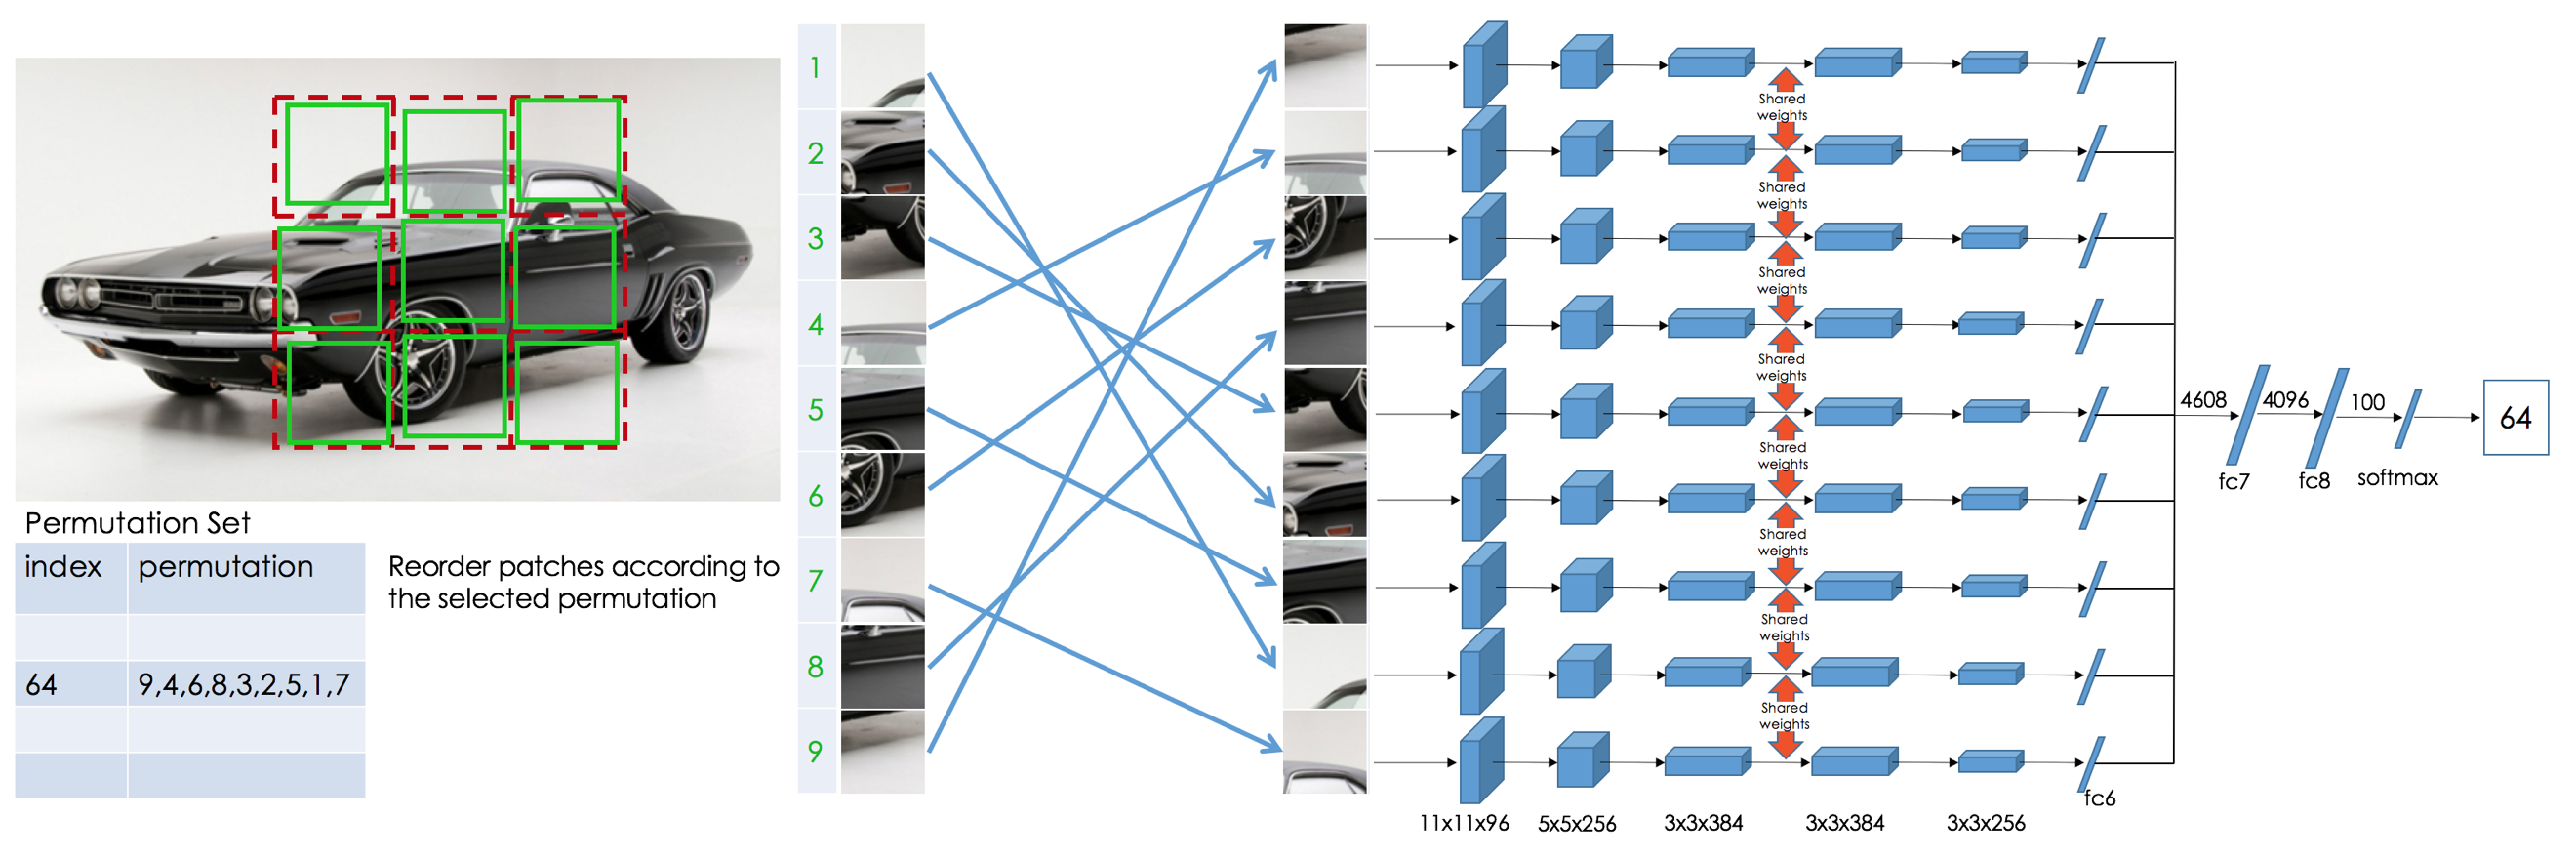
\includegraphics[width=1\textwidth]{Images/Chapter2/jigsaw.png}
\caption{ساختار کلی شبکه‌ی حل پازل}
\label{fig:jigsaw}
\end{figure}

مطالعه‌ی انجام‌شده در این مقاله نشان داد که مدل آموزش‌دیده با این وظیفه‌ی پوششی، قادر به یادگیری بازنمایی‌هایی با کیفیت بالا بوده که در وظایف پایین‌دستی همچون طبقه‌بندی تصویر و شناسایی اشیاء عملکرد قابل توجهی داشته‌اند. همچنین این روش راه را برای توسعه‌ی سایر وظایف زمینه‌محور در یادگیری خودنظارتی هموار ساخت و مبنایی برای کارهای بعدی\cite{li2021jigsawgan,park2024fine} در این حوزه شد. \newline

\noindent\textbf{وظیفه‌ی پوششی پیش‌بینی ترتیب صحیح در دنباله:}

یکی دیگر از وظایف پوششی مبتنی بر زمینه، وظیفه‌ی پیش‌بینی درستی یا نادرستی ترتیب زمانی فریم‌های یک ویدیو است. این وظیفه نخستین بار توسط میسرا و همکارانش در مقاله‌ای با عنوان \lr{Shuffle and Learn} \cite{misra2016shuffle} معرفی شد. ایده‌ی اصلی این روش آن است که فریم‌های استخراج‌شده از یک ویدیو را به‌صورت یک دنباله‌ی تصویری به مدل می‌دهیم و از آن انتظار داریم که تشخیص دهد آیا ترتیب زمانی این فریم‌ها حفظ شده است یا به‌طور تصادفی به هم ریخته شده‌اند. در واقع، این روش یک مسئله‌ی طبقه‌بندی دودویی را تعریف می‌کند که خروجی آن مشخص می‌سازد آیا دنباله‌ی ورودی طبیعی و معنادار است یا نه.

برای افزایش دشواری این وظیفه و در نتیجه به‌دست آوردن بازنمایی‌های باکیفیت‌تر، در مرحله‌ی انتخاب فریم‌ها، از یک راهبرد هوشمندانه بهره گرفته می‌شود. همانطور که در شکل \ref{fig:video-permutation} نشان داده شده است، فریم‌هایی از ویدیو انتخاب می‌شوند که دارای بیشترین تفاوت‌ بصری با یکدیگر هستند. این کار موجب می‌شود مدل نتواند صرفا بر پایه‌ی اطلاعات سطح پایین مانند رنگ یا بافت، تصمیم‌گیری کند، بلکه ناگزیر شود برای تشخیص ترتیب صحیح، به درک عمیق‌تری از محتوای ویدیویی و روابط زمانی میان فریم‌ها برسد.

\begin{figure}[htbp]
\centering
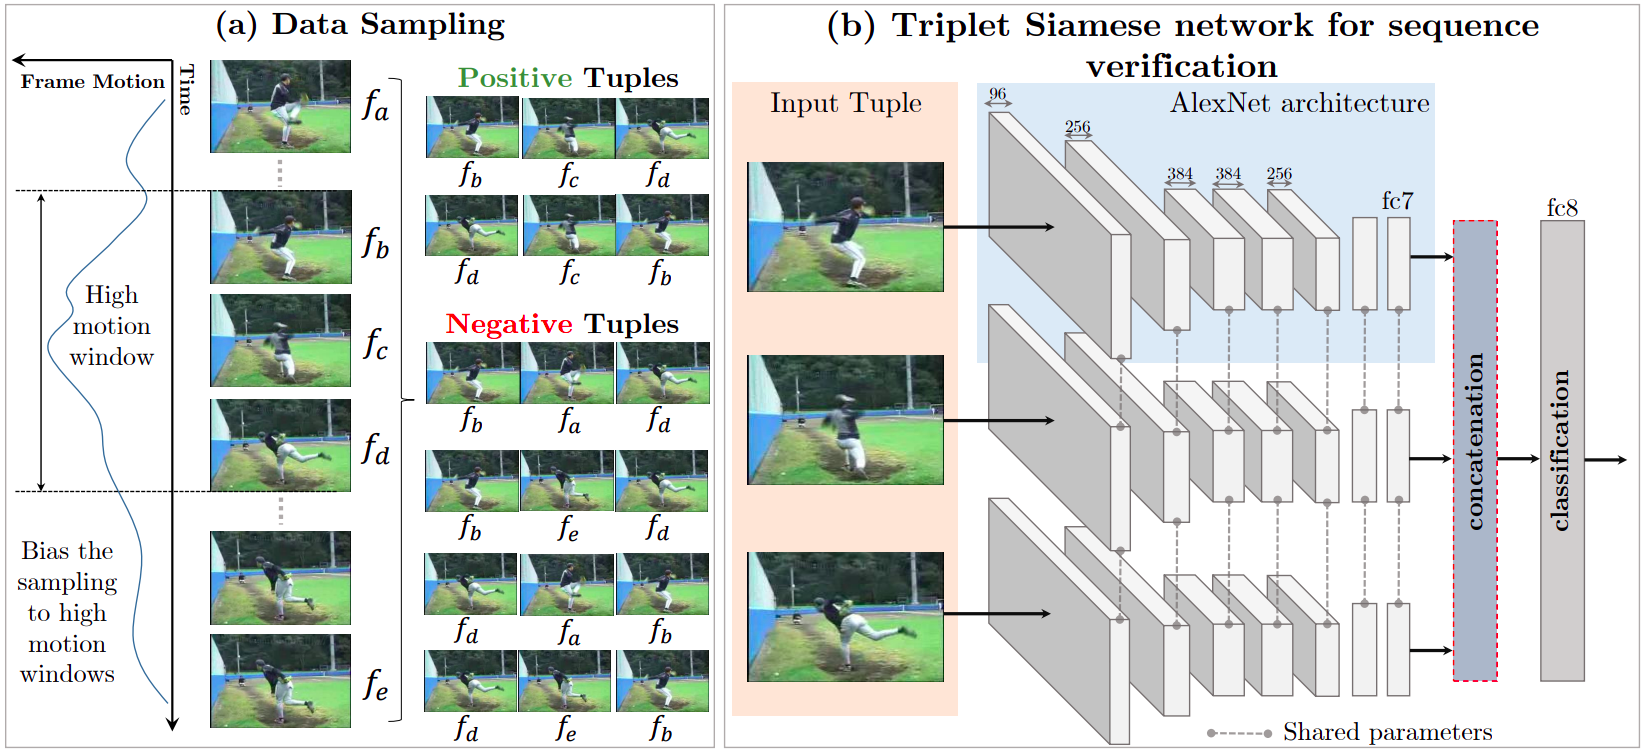
\includegraphics[width=1\textwidth]{Images/Chapter2/video-permutation.png}
\caption{ساختار کلی شبکه‌ی بررسی درستی ترتیب فریم‌های ویدیویی}
\label{fig:video-permutation}
\end{figure}

ساختار کلی شبکه‌ی مورد استفاده نیز شباهت زیادی به روش حل پازل تصویری دارد که پیش‌تر معرفی شد (شکل \ref{fig:jigsaw}). در اینجا نیز از یک شبکه‌ی عصبی برای استخراج ویژگی‌های هر فریم استفاده می‌شود و سپس ویژگی‌های استخراج‌شده در سطحی بالاتر با یکدیگر ترکیب می‌شوند تا تصمیم‌گیری نهایی صورت گیرد. اگرچه این دو روش در ظاهر شباهت‌های زیادی دارند، اما در عمل بر نوع داده‌های متفاوتی تکیه دارند (تصویر در برابر ویدیو) و همچنین اهداف طبقه‌بندی‌شان نیز تفاوت دارد (تشخیص ترتیب صحیح در برابر پیش‌بینی جایگشت دقیق).

علاوه بر داده‌های ویدیویی، این رویکرد در حوزه‌های غیرتصویری نیز مورد استفاده قرار گرفته است. برای مثال مطالعاتی بر روی سیگنال‌های مغزی ثبت‌شده با استفاده از الکتروانسفالوگرافی\footnote{الکتروانسفالوگرافی یا نوار مغزی، روشی برای ثبت فعالیت الکتریکی مغز است. در این روش الکترودهایی بر روی پوست سر قرار داده می‌شوند تا امواج مغزی را ثبت کرده و به تشخیص اختلالاتی مانند صرع، مشکلات خواب و آسیب‌های مغزی کمک کنند} (\lr{EEG}) انجام شده که یادگیری خودنظارتی را بر روی سیگنال‌های \lr{EEG} تعمیم می‌دهد\cite{weng2025self}.
ایده‌ی تشخیص ترتیب زمانی را به داده‌های چندکاناله‌ی \lr{EEG} این کار نشان می‌دهد که وظایف پوششی مبتنی بر ترتیب، نه تنها در داده‌های بصری، بلکه در داده‌های زمانی پیچیده نیز قابل کاربرد و اثربخش هستند.

\subsubsection{روش‌های بازسازی‌محور}

حال به سراغ دسته‌ی دیگری از روش‌های وظایف پوششی تحت عنوان بازسازی‌محور می‌رویم. در این دسته، ایده‌ی اصلی آن است که مدل با مشاهده‌ی بخشی از داده، یا نسخه‌ای ناقص، فشرده یا مخدوش‌شده‌ی آن، تلاش کند نسخه‌ی کامل یا اصلی داده را بازسازی کند. این فرایند باعث می‌شود مدل ناگزیر به استخراج اطلاعات بنیادی و ساختاری از داده باشد. روش‌های بازسازی‌محور، به‌ویژه در یادگیری نمایش‌های عمیق و قابل انتقال، اهمیت زیادی دارند و بسیاری از آن‌ها با روش‌های مولد نیز همپوشانی دارند؛ چراکه در هر دو، بازتولید داده نقش کلیدی دارد.\newline


\noindent\textbf{ترمیم تصویر:}

وظیفه پوششی ترمیم تصویر\LTRfootnote{Image Inpainting}
که توسط پاتاک و همکاران\cite{pathak2016context}
ارائه شد، از خودکدگذاری تحت عنوان
کدگذار زمینه‌ای\LTRfootnote{Context Encoder}
استفاده می‌کند تا بتواند یک شبکه‌ی پیچشی را طوری آموزش دهد که بخش‌های حذف‌شده و آسیب‌دیده از تصویر را بازسازی و ترمیم نماید. شبکه برای این که بتواند این وظیفه را به خوبی انجام دهد باید توانایی درک مفاهیم موجود در داده را داشته باشد.
در شکل \ref{fig:inpainting-losses}
یک نمونه از عملکرد این روش را با استفاده از دو تابع هزینه‌ی مختلف می‌توان دید.

\begin{figure}[htb!]
\centering
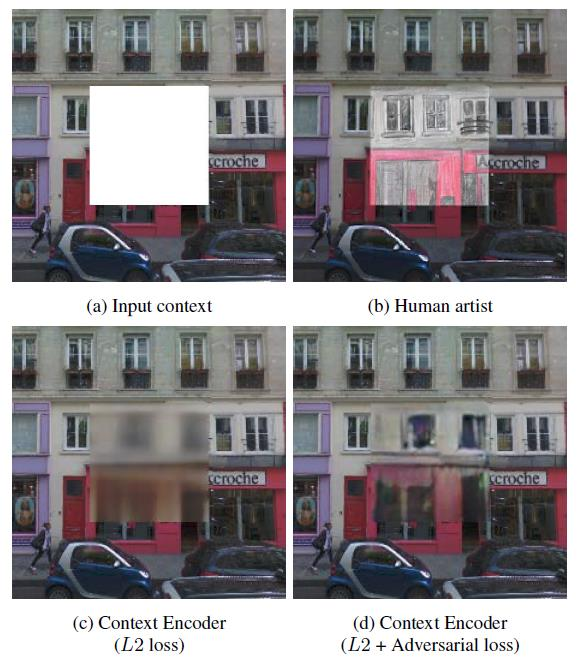
\includegraphics[width=0.7\textwidth]{Images/Chapter2/inpainting-losses.png}
\caption{عملکرد کدگذار زمینه‌ای برای ترمیم تصاویر}
\label{fig:inpainting-losses}
\end{figure}

معماری کلی کدگذار زمینه‌ای این‌گونه است که ابتدا یک یا چند ناحیه از تصاویر را به صورت تصادفی حذف می‌کنیم. این نواحی تصادفی می‌توانند انواع اشکال هندسی مانند دایره و مربع و یا حتی کاملا تصادفی باشد. سپس این تصویر تخریب شده به ورودی شبکه‌ی رمگذار داده می‌شود که معماری کلی آن شباهت زیادی به شبکه‌ی
\lr{AlexNet}
دارد. شبکه‌ی کدگذار یک ماتریس به فرم
$C \times W \times H$
به ازای هر نمونه می‌دهد که در آن $C$ بیانگر تعداد کانال‌ها و $W$ و $H$ بیانگر عرض و ارتفاع ماتریس خروجی هستند. در معماری شبکه‌ی کدگذار زمینه‌ای، برای افزایش ظرفیت یادگیری مدل، خروجی مدل مستقیما به رمزگشا داده نمی‌شود. بلکه از یک لایه‌ی تمام متصل استفاده می‌شود. برای استفاده از لایه‌ی تماما متصل معمولا از
روش‌های ادغام\LTRfootnote{Pooling Methods}
مانند ادغام حداکثر استفاده می‌شود. این‌گونه ابعاد از
$C \times W \times H$
به $C$ تغییر می‌کند.
اما ایراد ادغام این است که می‌تواند اطلاعات باارزش را از بین ببرد. علاوه بر آن اگر بخواهیم که بدون استفاده از ادغام از لایه‌ی تماما متصل استفاده کنیم، باید خروجی را به فرم برداری به طول
$C \times W \times H$
درآوریم که حدود ۱۰۰ میلیون پارامتر به شبکه اضافه می‌کند. این کار علاوه بر پردازش پیچیده، مشکل بیش‌برازش را نیز به‌دنبال خواهد داشت. به‌همین منظور محققان در این مقاله از یک لایه‌ی
تماما متصل درون‌کانالی\LTRfootnote{Channel-wise Fully Connected}
استفاده کردند. بدین صورت که هر یک از
$C$
کانال را به یک بردار به طول
$W \times H$
تبدیل می‌کنیم. سپس یک لایه خواهیم داشت که در دل خود
$C$
لایه‌ی تمام متصل مانند شکل \ref{fig:inpainting-architecture} دارد.
نتیجتا خروجی کدگذار به ورودی رمزگشا همراه با یک لایه‌ی غیر خطی متصل خواهد شد، اطلاعاتی از بین نخواهد رفت و تعداد پارامترهای قابل یادگیری مقدار اندکی افزایش خواهند یافت که برای ما قابل تحمل هستند.

\begin{figure}[htb!]
\centering
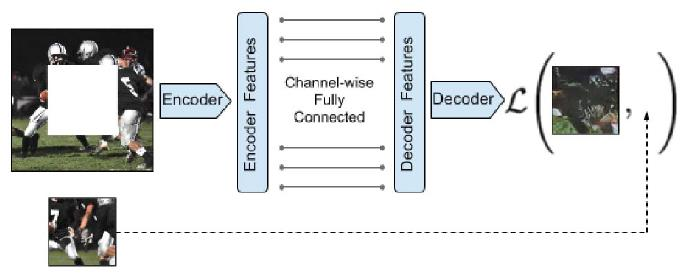
\includegraphics[width=1.0\textwidth]{Images/Chapter2/inpainting-architecture.png}
\caption{معماری کدگذار زمینه‌ای}
\label{fig:inpainting-architecture}
\end{figure}

در رمزگشا با استفاده از لایه‌های
پیچشی معکوس\footnote{منظور از «لایه‌ی پیچشی معکوس»، همان عملیات
\lr{transposed convolution} یا \lr{deconvolution}
است که برای بزرگ‌نمایی ویژگی‌ها در شبکه‌های مولد یا رمزگشا به‌کار می‌رود.}،
ویژگی‌های فشرده شده را به ابعاد تصویر ورودی می‌رسانیم. مثلا ویژگی‌های ورودی به رمزگشا اگر دارای ۶۴ کانال با طول و عرض ۱۶ باشند، آن را به ۳ کانال با طول و عرض ۲۵۶ می‌رسانیم. سپس سیگنال نظارت که همان تصویر سالم است اعمال می‌شود و با استفاده از یک تابع هزینه، آموزش شبکه انجام می‌شود. تابع هزینه‌ی ابتدایی،
میانگین مربعات خطا (\lr{MSE}\LTRfootnote{Mean Squared Error}
می‌باشد
که در فرمول \ref{eq:mse} قابل مشاهده است.
\begin{equation}
    \label{eq:mse}
    L_{rec}(x) = \| \hat{M} \odot (x - F((1 -   \hat{M}) \odot x)) \|_2
\end{equation}
اما همانطور که در شکل \ref{fig:inpainting-losses} بخش \lr{c}
قابل مشاهده است، این تابع هزینه یک خروجی محو شده به ما می‌دهد. محققان برای بهبود خروجی تولید شده از تابع هزینه‌ی تخاصمی استفاده کردند. در واقع از یک شبکه‌ی اضافه تحت عنوان
تفکیک‌کننده\LTRfootnote{Discriminator}
بر پایه‌ی شبکه‌ی مولد تخاصمی استفاده کردند. در اینجا خروجی رمزگشا حکم مولد را خواهد داشت. بنابراین فرمول‌بندی آن به فرم فرمول \ref{eq:adversarial} در می‌آید.
البته در نهایت از ترکیب هزینه‌ی \lr{mse}
و تخاصمی استفاده می‌شود که به فرم فرمول
\ref{eq:combined}
نهایی می‌شود. همانطور که در شکل
\ref{fig:inpainting-losses}
بخش \lr{d}
نیز دیده می‌شود، خروجی دقیق‌تر و بهتری به‌دست می‌آید.
\begin{equation}
    \label{eq:adversarial}
    L_{adv} = \max_{D} \mathbb{E}_{x \in X} [\log(D(x)) + \log(1 - D(F((1 - \hat{M}) \odot x)))]
\end{equation}
\begin{equation}
    \label{eq:combined}
    L = \lambda_{rec} L_{rec} + \lambda_{adv} L_{adv}
\end{equation}
در مقاله، مقدار
$\lambda_{adv}$ برابر با
$0.001$ و مقدار $\lambda_{rec}$ برابر با
$0.999$ قرار داده شده است.
بنابراین هدف اصلی بازتولید دقیق تصویر می‌باشد اما مقدار کمی هزینه‌ی تخاصمی نیز برای وضوح تصاویر تولید شده استفاده شده است.

روش ترمیم تصویر با استفاده از کدگذار زمینه‌ای علاوه بر اینکه وظیفه‌ی اصلی خود یعنی بازسازی نواحی حذف‌شده را انجام می‌دهد، به عنوان یک سیستم پیش‌آموزش قدرتمند برای استخراج ویژگی‌های بصری نیز عمل می‌کند. در حقیقت پس از آموزش کدگذار روی تصاویر بدون برچسب، می‌توان آن را بر روی یک مجموعه داده‌ی دارای برچسب تنظیم دقیق کرد و وظایفی مانند دسته‌بندی را انجام داد.

\subsubsection{یادگیری تباینی}

با وجود پیشرفت‌هایی که روش‌های پیشین یادگیری خودنظارتی در زمان خود به همراه داشتند، همچنان عملکرد آن‌ها فاصله‌ی محسوسی با روش‌های نظارت‌شده کامل داشت. این شکاف عملکردی تا حد زیادی با ظهور یادگیری تباینی در چارچوب یادگیری خودنظارتی کاهش یافت. بهره‌گیری از ایده‌های تباینی منجر به رشد قابل‌توجهی در کیفیت بازنمایی‌های استخراج‌شده از داده‌ها شد، به‌طوری‌که عملکرد مدل‌های بدون‌نظارت در برخی وظایف به سطوح قابل‌مقایسه‌ای با روش‌های نظارت‌شده رسید. در سال‌های اخیر، تمرکز بسیاری از مقالات بر توسعه و بهبود روش‌های خودنظارتی تباینی بر روی انواع داده‌های مختلف از جمله تصویر و سیگنال بوده است. در ادامه، ابتدا به شرح مفهوم یادگیری تباینی پرداخته و سپس برخی از روش‌های شاخص مبتنی بر این رویکرد را مرور می‌کنیم.\newline

\noindent\textbf{تعریف یادگیری تباینی}

یادگیری تباینی در بستر یادگیری خودنظارتی، رویکردی مبتنی بر تمایز است که تلاش می‌کند بازنمایی‌هایی مشابه برای نمونه‌های با مفهوم یکسان و بازنمایی‌هایی متمایز برای نمونه‌های ناهم‌معنا ایجاد کند. این امر معمولاً با بهره‌گیری از تکنیک‌های داده‌افزایی محقق می‌شود؛ به‌این‌ترتیب که از یک داده‌ی واحد چندین نسخه‌ی تغییریافته تولید شده و به‌عنوان نمونه‌های «مثبت» در نظر گرفته می‌شوند، در حالی که داده‌های متفاوت، نمونه‌های «منفی» تلقی می‌گردند. هدف از آموزش مدل، نزدیک کردن بازنمایی نمونه‌های مثبت به یکدیگر و دور ساختن آن‌ها از نمونه‌های منفی است.

برای مثال، فرض کنید از مجموعه داده، دو نمونه‌ی $A$ و $B$ انتخاب می‌شوند و سپس با اعمال داده‌افزایی، نمونه‌های $A_1$ و $B_1$ از آن‌ها ساخته می‌شوند. مدل باید یاد بگیرد که $A$ و $A_1$ را به‌عنوان نمونه‌های مشابه و $A$ و $B_1$ را به‌عنوان نمونه‌های متفاوت در نظر بگیرد. این فرایند با تعریف یک تابع هزینه بر پایه‌ی بردارهای بازنمایی حاصل از یک کدگذار پیاده‌سازی می‌شود (شکل \ref{fig:contrastive}) \cite{jaiswal2020survey}. در نهایت، کدگذار آموزش‌دیده قادر خواهد بود بازنمایی‌هایی غنی و قابل‌انتقال برای استفاده در وظایف یادگیری پایین‌دستی فراهم آورد.

\begin{figure}[htb!]
\centering
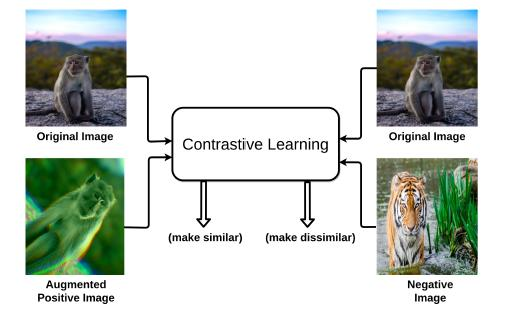
\includegraphics[width=0.7\textwidth]{Images/Chapter2/contrastive.png}
\caption{نمونه‌ای از فرایند یادگیری تباینی}
\label{fig:contrastive}
\end{figure}

در ادامه به بررسی تعدادی از روش‌ها و مقالات منتشر شده در این حوزه می‌پردازیم.\newline

\noindent\textbf{روش کدگذاری پیش‌بینی‌کننده‌ی تباینی (\lr{CPC\LTRfootnote{Contrastive Predictive Coding}})}\label{sec:CPC}

روش کدگذاری پیش‌بینی‌کننده‌ی تباینی یا به اختصار \lr{CPC}
که نخستین بار در سال ۲۰۱۸ توسط
\lr{Oord}
و همکاران\cite{oord2018representation}
معرفی شد، یکی از اولین تلاش‌های موفق برای استفاده از یادگیری تباینی در استخراج بازنمایی‌های غنی و قابل انتقال از داده‌های بدون برچسب بود. این روش، به‌ویژه در داده‌های ترتیبی مانند صوت و سیگنال، عملکرد قابل‌توجهی از خود نشان داده و در حوزه‌هایی مانند تشخیص گفتار کاربرد یافته است.

ایده‌ی اصلی این روش بر پایه‌ی پیش‌بینی اطلاعات آینده از روی گذشته است. اما بر خلاف بسیاری از دیگر روش‌های
خودهمبسته\LTRfootnote{Autoregressive}
که آینده را با تولید داده‌ی اصلی پیش‌بینی می‌کنند، یک مدل مولد نیست. بلکه یک مدل تباینی است که هدف آن پیش‌بینی بازنمایی مربوط به آینده با استفاده از تابع هزینه تباینی است.

\begin{figure}[htb!]
\centering
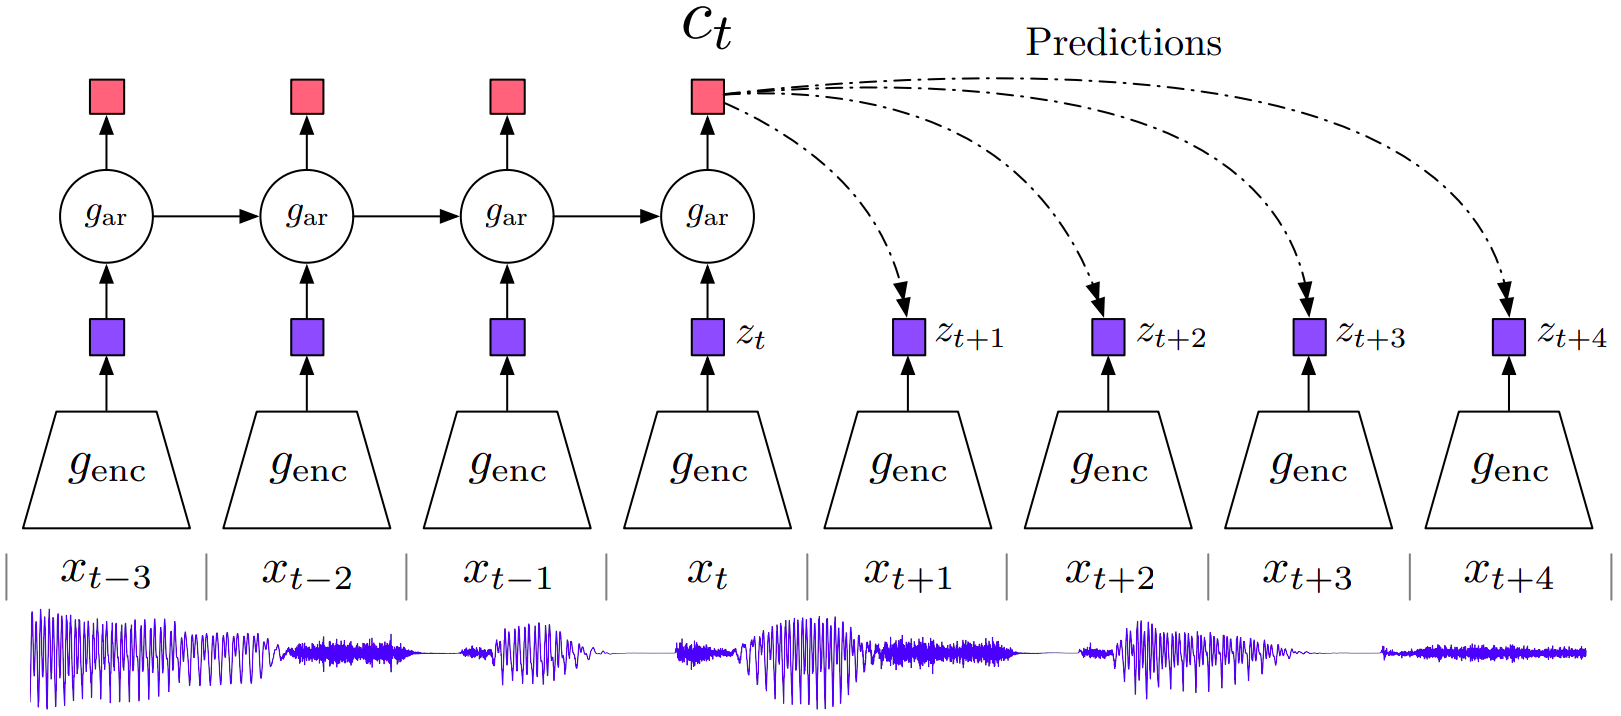
\includegraphics[width=1\textwidth]{Images/Chapter2/cpc.png}
\caption{ساختار کلی روش \lr{CPC}}
\label{fig:cpc}
\end{figure}

با این فرض که مجموعه داده ورودی سری زمانی می‌باشد،
فرض کنید در $x_t$ هستیم
که هر $x_t$
بیانگر یک پنجره از سری زمانی می‌باشد که می‌تواند دارای همپوشانی با پنجره‌های مجاور باشد. با استفاده از یک شبکه‌ی پیچشی ($g_{enc}$)، بردارهای بازنمایی برای پنجره‌های از
$x_{t-n}$ تا $x_t$ می‌سازیم.
سپس با استفاده از یک شبکه‌ی بازگشتی مانند واحد بازگشتی دروازه‌ای ($g_{ar}$)،
از روی
$g_{enc}(x_{t-n})$ تا $g_{enc}(x_t)$
یک بردار زمینه تحت عنوان $c_t$
تولید می‌کنیم.

حال به نوآوری این روش می‌رسیم. در روش \lr{CPC}
به‌جای این که از بردار $c_t$
برای تخمین مستقیم توزیع احتمالاتی $k$ قدم آینده استفاده شود
(یعنی $p_k(x_{t+k}|c_t)$)،
از یک نسبت چگالی\LTRfootnote{Density Ratio}
استفاده می‌شود که هدف آن حفظ اطلاعات متقابل بین بازنمایی آینده
$z_{t+k}$ و بردار زمینه $c_t$ است.
این نسبت چگالی به‌صورت معادله \ref{eq:density-ratio} مدل‌سازی می‌شود
که در آن تابع امتیازدهی $f_k$
میزان شباهت بازنمایی آینده و زمینه را نشان می‌دهد. برای پیاده‌سازی، از یک مدل ساده به فرم
معادله \ref{eq:density-ratio-simple}
استفاده شده است که در آن $W_k$
یک ماتریس تبدیل خطی قابل آموزش برای گام زمانی $k$ است.
این مدل با محاسبه‌ی شباهت بین بردار
$z_{t+k}$
(که یک نماینده‌ی بازنمایی برای آینده است)
و بردار زمینه‌ی $c_t$،
تلاش می‌کند که امتیاز را برای
$z_{t+k}$های مثبت بیشینه
و برای $z_{t+k}$های منفی کمینه کند
\begin{equation}
\label{eq:density-ratio}
f_k(z_{t+k}, c_t) \propto \frac{p(z_{t+k}|c_t)}{p(z_{t+k})}
\end{equation}
\begin{equation}
\label{eq:density-ratio-simple}
f_k(z_{t+k}, c_t) = \exp \left( z_{t+k}^T W_k c_t \right)
\end{equation}
برای آموزش مدل، از تابع هزینه‌ی
\lr{InfoNCE\LTRfootnote{Information Noise-Contrastive Estimation}} به فرم معادله‌ی \ref{eq:infonce}
استفاده می‌شود که در آن $X$ شامل $N$
نمونه‌ی تصادفی است که یکی از آن‌ها نمونه‌ی مثبت و $N-1$
تای دیگر نمونه‌های منفی هستند. هدف مدل این است که امتیاز شباهت $f_k$
برای نمونه‌ی واقعی نسبت به نمونه‌های منفی بیشتر باشد. بدین ترتیب، مدل می‌آموزد که بازنمایی $c_t$
شامل اطلاعات مفیدی برای پیش‌بینی آینده‌ی داده باشد.
\begin{equation}
\label{eq:infonce}
\mathcal{L}_N = - \mathbb{E}_X \left[ \log \frac{f_k(x_{t+k}, c_t)}{\sum_{x_j \in X} f_k(x_j, c_t)} \right]
\end{equation}
در نهایت، پس از پایان مرحله‌ی پیش‌‌آموزش، می‌توان از کدگذار آموزش‌دیده به‌عنوان یک استخراج‌کننده‌ی ویژگی استفاده کرد و بازنمایی‌های به‌دست‌آمده را در وظایف پایین‌دستی مانند دسته‌بندی به‌کار برد.\newline

\noindent\textbf{استفاده از بانک حافظه\LTRfootnote{Memory Bank} و تکانه\LTRfootnote{Momentum}:}

یکی از چالش‌های اصلی در پیاده‌سازی موثر یادگیری تباینی، نیاز به مجموعه‌ای بزرگ و متنوع از نمونه‌های منفی است. برای اینکه مدل بتواند تمایز درستی بین نمونه‌های مثبت و منفی قائل شود، باید در هر تکرار آموزشی تعداد زیادی نمونه‌ی منفی داشته باشد. این در حالی است که در یک دسته از ورودی، تنها تعداد محدودی از نمونه‌ی منفی در دسترس است. به همین منظور، محققان روشی تحت عنوان
بانک حافظه\cite{wu2018unsupervised}
را ارائه دادند.

در این روش، به‌جای آن که فقط از داده‌های موجود در دسته‌ی ورودی فعلی استفاده شود، یک بردار بازنمایی برای هر نمونه در کل مجموعه داده محاسبه و در یک بانک حافظه ذخیره می‌شود. در طول آموزش، این بانک به‌طور تدریجی به‌روزرسانی شده و از آن برای استخراج نمونه‌های منفی استفاده می‌شود. فرض اصلی این روش (مانند بیشتر روش‌های دیگر تباینی) این است که هر نمونه در مجموعه داده به‌عنوان یک کلاس منحصربه‌فرد در نظر گرفته شود و بنابراین یادگیری بازنمایی به‌صورت تباینی بر اساس تفاوت بین نمونه‌ها صورت می‌گیرد.
\begin{equation}
\label{eq:membank-infonce}
\mathcal{L}_i = -\log \frac{\exp(z_i^\top v_i / \tau)}{\sum_{j=1}^{K} \exp(z_i^\top v_j / \tau)}
\end{equation}

تابع هزینه به‌کاررفته در این روش به فرم معادله‌ی \ref{eq:membank-infonce}
می‌باشد که همان تابع هزینه‌ی \lr{InfoNCE}
می‌باشد. در این فرمول:
\begin{itemize}
    \item $z_i$ بردار بازنمایی نمونه‌ی ورودی است که توسط شبکه کدگذار تولید شده است.
    \item $v_i$ بازنمایی ذخیره شده‌ی همان نمونه در بانک حافظه است (مثبت).
    \item $v_j$ دیگر نمونه‌های استخراج‌شده از بانک حافظه‌اند.
    \item $\tau$ پارامتر دما است که بسته به مقدار آن باعث هموارسازی یا تیزکردن نمودار خروجی می‌شود.
\end{itemize}
با وجود عملکرد قابل قبول، یکی از مشکلات این روش آن است که بانک حافظه به‌صورت مستقیم از پارامترهای کدگذار فعلی به‌روزرسانی نمی‌شود و در طول آموزش بین بازنمایی‌های فعلی و آنچه در حافظه ذخیره شده، ناسازگاری‌هایی به‌وجود خواهد آمد. این موضوع می‌تواند مانع از یادگیری پایدار شود.

در راستای رفع مشکل ناهماهنگی بانک حافظه، روش تباین تکانه یا به اختصار
\lr{Moco\LTRfootnote{Momentum Contrast}}
توسط \lr{He} و همکاران\cite{he2020momentum} معرفی شد.
ایده‌ی اصلی این روش استفاده از دو شبکه کدگذار است؛
یک کدگذار جستار\LTRfootnote{Query Encoder}
و یک کدگذار کلید\LTRfootnote{Key Encoder}.
کدگذار جستار مستقیما از طریق پس‌انتشار به‌روزرسانی می‌شود؛ در حالی که کدگذار کلید با استفاده از به‌روزرسانی تکانه‌ای روی کدگذار جستار به‌روزرسانی می‌شود. فرم به‌روزرسانی تکانه‌ای برای پارامترهای کدگذار کلید به شکل زیر تعریف می‌شود:
\begin{equation}
\theta_k \leftarrow m \cdot \theta_k + (1 - m) \cdot \theta_q
\end{equation}
که در آن:
\begin{itemize}
    \item $\theta_q$ پارامترهای کدگذار جستار است.
    \item $\theta_k$ پارامترهای کدگذار کلید است.
    \item $m$ ضریب تکانه است که با قرار دادن مقادیر نزدیک به ۱ (در مقاله برابر با $0.999$ می‌باشد) باعث می‌شود تغییرات پارامترهای کلید آهسته‌تر و پیوسته‌تر باشد.
\end{itemize}
\begin{figure}[htb!]
\centering
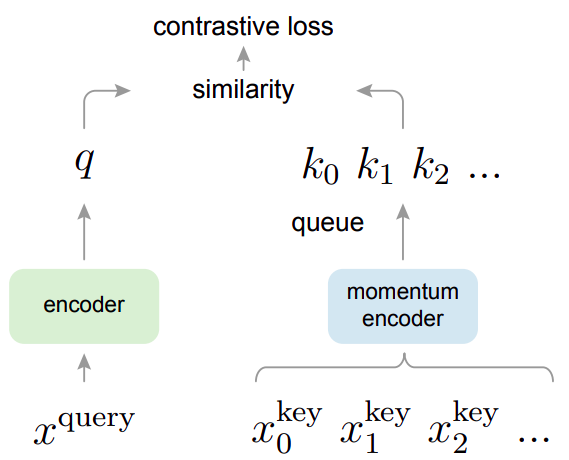
\includegraphics[width=0.6\textwidth]{Images/Chapter2/moco.png}
\caption{ساختار کلی روش \lr{MoCo}}
\label{fig:moco}
\end{figure}
از طرفی، \lr{MoCo}
به‌جای استفاده از یک بانک حافظه‌ی کامل که تمام داده‌ها را نگهداری می‌کند،
از یک صف حافظه\LTRfootnote{Queue}
استفاده می‌کند. در این صف، بازنمایی‌های کلید تولید شده از نمونه‌های قبلی ذخیره می‌شوند. به‌مرور زمان، نمونه‌های قدیمی از صف خارج شده و نمونه‌های جدید جای آن‌ها را می‌گیرند. این ساختار حافظه‌ی پویا، ضمن صرفه‌جویی در حافظه، امکان دسترسی به هزاران نمونه‌ی منفی را در هر تکرار آموزشی فراهم می‌کند. تابع هزینه مورد استفاده در \lr{MoCo}
نیز نوعی از \lr{InfoNCE} است:
\begin{equation}
\mathcal{L}_q = -\log \frac{\exp(q \cdot k^+ / \tau)}{\sum_{i=0}^{K} \exp(q \cdot k_i / \tau)}
\end{equation}
که در آن:
\begin{itemize}
    \item $q$ بازنمایی حاصل از کدگذار جستار است.
    \item $k^+$ نمونه‌های مثبت تولید شده توسط کدگذار کلید است
    \item $k_i$ نمونه‌های منفی ذخیره‌شده در صف حافظه هستند.
    \item $\tau$ پارامتر دما است.
\end{itemize}
روش \lr{MoCo}
به‌دلیل استفاده از کدگذار کلید با به‌روزرسانی تکانه‌ای، انسجام میان بازنمایی‌های فعلی و نمونه‌های منفی ذخیره‌شده را حفظ می‌کند و در عین حال بدون نیاز به پردازش مجدد تمام داده‌ها، بازنمایی‌های به‌روز و موثری تولید می‌نماید. این مدل باعث پایداری بیشتر آموزش و بهبود دقت مدل‌های پیش‌آموزش‌یافته شد.\newline

\noindent\textbf{یادگیری تباینی ساده اما قدرتمند: روش \lr{SimCLR}}\label{sec:simclr}

روش یادگیری تباینی ساده که به‌اختصار
\lr{SimCLR\LTRfootnote{Simple Framework for Contrastive Learning of Visual Representations}}
نامیده می‌شود، یکی از اثرگذارترین و پایه‌ای‌ترین روش‌های یادگیری تباینی خودنظارتی است که توسط
چن و همکاران\cite{chen2020simple}
معرفی شد. برخلاف روش‌هایی مانند
\lr{MoCo}
که به ساختارهای پیچیده‌ای نظیر صف حافظه و کدگذار تکانه‌ای نیاز دارند،
\lr{SimCLR}
با ساختاری بسیار ساده، توانست بازنمایی‌های قدرتمندی را برای تصاویر یاد بگیرد و عملکرد قابل مقایسه با روش‌های نظارت‌شده به‌دست آورد. سادگی معماری در کنار داده‌افزایی قوی و دسته‌های بزرگ داده آموزشی کلید عملکرد خوب این روش است.

فرایند آموزش در \lr{SimCLR}
از چهار جزء اصلی تشکیل شده است:
\begin{enumerate}
    \item داده‌افزایی قوی
    \item شبکه کدگذار
    \item شبکه نگاشت\LTRfootnote{Projection Head}
    \item تابع هزینه \lr{InfoNCE}
\end{enumerate}

در ادامه هر یک از این اجزا را بررسی می‌کنیم.

\noindent\textbf{داده‌افزایی قوی:}
دو تابع داده‌افزایی به‌صورت تصادفی بر روی هر ورودی $xـk$
اعمال می‌شود و در نتیجه‌ی آن دو نمایش
$x_{2k-1}$ و $x_{2k}$ تولید می‌گردند.
ترکیب‌های متعددی از تابع‌های تبدیل مختلف موجود در شکل
\ref{fig:simclr-augmentations}
به‌صورت تصادفی می‌توانند استفاده شوند تا خروجی‌های مختلف و تصادفی برای هر داده ایجاد شوند. برای مثال یکی از توابع مورد استفاده می‌تواند به‌این صورت باشد که با یک احتمال برش انجام دهد، با یک احتمال تصویر را قرینه و برعکس کند، نویز تصادفی گوسی با میانگین
$\mu$ و انحراف معیار $\sigma$
اعمال کند و رنگ تصویر را به‌صورت تصادفی تغییر دهد. نتیجتا با دو بار اعمال این تابع تصادفی بر روی هر ورودی، دو داده‌ی افزوده خواهیم داشت که باید شباهتشان را با یکدیگر بیشینه کنیم. هر چه شدت اعمال روش‌های افزایش داده بیشتر باشد، تفکیک بین داده‌های مثبت و منفی را برای مدل سخت‌تر می‌کند؛ اما همین امر می‌تواند باعث شود که مدل وادار به یادگیری بازنمایی‌های مفیدتر و کاربردی‌تر شود. همچنین هر چه تعداد نمونه‌های منفی درون یک دسته‌ی آموزشی بیشتر باشد، مدل نمونه‌های بیشتری را می‌بیند و به‌همین ترتیب تباین بهتری می‌تواند انجام دهد و یادگیری قوی‌تر و پایدارتر می‌شود.
\begin{figure}[t!]
\centering
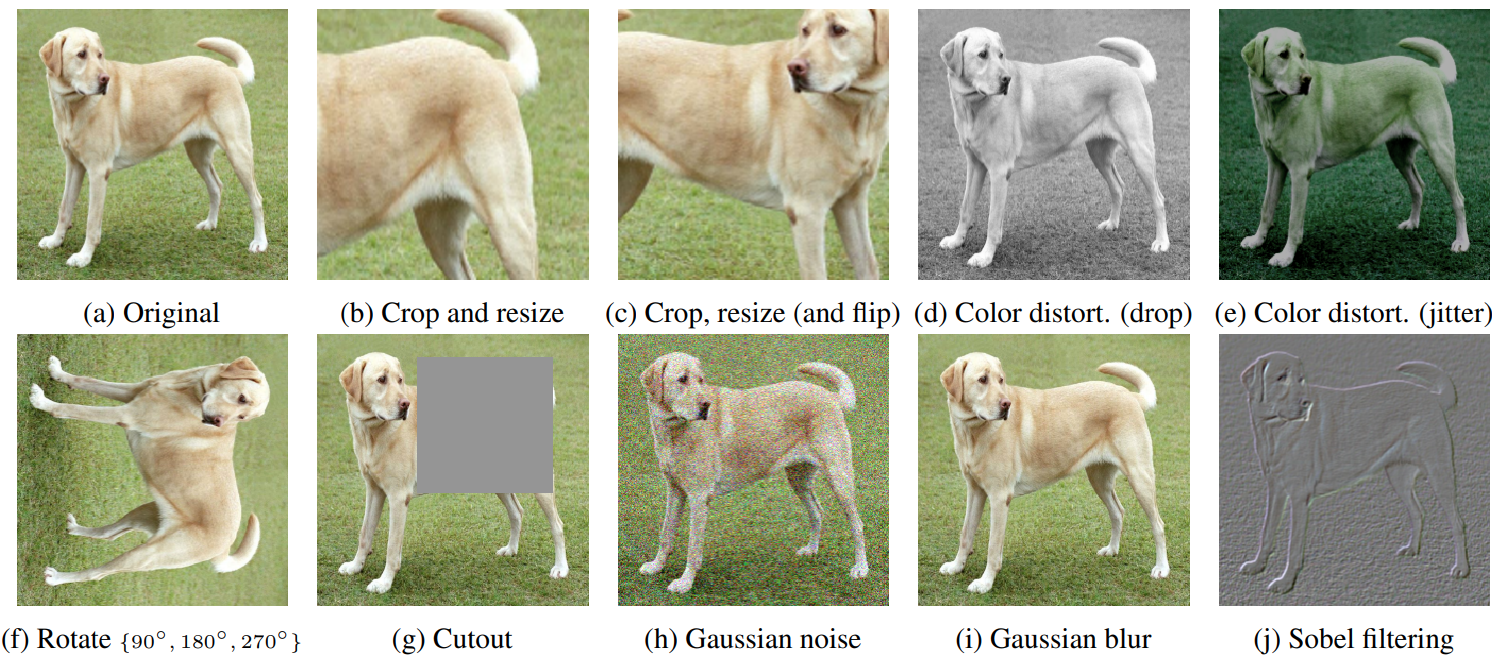
\includegraphics[width=1\textwidth]{Images/Chapter2/simclr-augmentations.png}
\caption{روش‌های ایجاد داده‌ی افزوده}
\label{fig:simclr-augmentations}
\end{figure}

\noindent\textbf{شبکه کدگذار:}
برای هر نما $x_\ell$،
با استفاده از کدگذار $f_\theta$ مبتنی بر شبکه‌ی پیچشی،
یک بردار بازنمایی $h_\ell$
به فرم معادله \ref{eq:simclr-encoder} می‌سازیم.
\begin{equation}
\label{eq:simclr-encoder}
h_\ell = f_\theta(x_\ell)\in\mathbb{R}^d
\end{equation}
در مقاله، از یک شبکه \lr{ResNet}
بدون لایه‌ی دسته‌بندی کننده استفاده شده است و
$h_\ell$
بعد از تجمیع سراسری به‌دست می‌آید. در ارزیابی پایین‌دستی از همین $h$
به‌عنوان بازنمایی نهایی برای هر نمونه استفاده می‌شود.

\noindent\textbf{شبکه نگاشت:}
یکی از نوآوری‌های روش \lr{SimCLR}،
استفاده از یک شبکه تماما متصل کم‌عمق (یک لایه پنهان) تحت عنوان شبکه نگاشت می‌باشد. با استفاده از این شبکه، خروجی $h_\ell$
تبدیل به $z_\ell$ می‌شود.
\begin{equation}
\label{eq:simclr-projection}
\boldsymbol{z}_\ell = g_\phi(\boldsymbol{h}_\ell) = \boldsymbol{W}^{(2)} \sigma(\boldsymbol{W}^{(1)} \boldsymbol{h}_\ell)
\end{equation}
نویسندگان مقاله نشان دادند که استفاده از یک شبکه نگاشت و یک تابع فعال‌ساز غیر خطی و سپس اعمال هزینه‌ی تباینی بر روی
$z$
عملکرد بهتری را نسبت به استفاده از
$h$
برای محاسبات هزینه‌ی تباینی می‌دهد. ایده‌ی شهودی برای این کار این است که
$g_\phi$
جذب‌کننده‌ی هزینه‌ی تباینی باشد تا
$f_\theta$
بازنمایی‌های عمومی‌تری را بیاموزد.
در معادله \ref{eq:simclr-projection}،
$W^{(1)}$ و $W^{(2)}$ پارامترهای شبکه‌ی نگاشت و
$\sigma$ تابع فعال‌ساز غیر خطی می‌باشد که معمولا از تابع \lr{ReLU\LTRfootnote{Rectified Linear Unit}} استفاده می‌شود.

\noindent\textbf{تابع هزینه تباینی:}
فرض کنید یک دسته آموزشی شامل $N$
نمونه ورودی باشد. پس با دو نما از هر تصویر،
$2N$
نمونه آموزشی خواهیم داشت. سپس برای دو نمونه‌ی مثبت $i$ و $j$ معادله
\ref{eq:simclr-loss} را خواهیم داشت.
\begin{equation}
\label{eq:simclr-loss}
    \ell_{i,j} = -\log \frac{\exp(sim(\boldsymbol{z}_i, \boldsymbol{z}_j) / \tau)}{\sum_{k=1}^{2N} 1_{[k \neq i]} \exp(sim(\boldsymbol{z}_i, \boldsymbol{z}_k) / \tau)}
\end{equation}
\begin{equation}
    \label{eq:simclr-cosine}
    sim(\boldsymbol{u}, \boldsymbol{v}) = \boldsymbol{u}^\top \boldsymbol{v} / \|\boldsymbol{u}\| \|\boldsymbol{v}\|
\end{equation}
\begin{figure}[t]
\centering
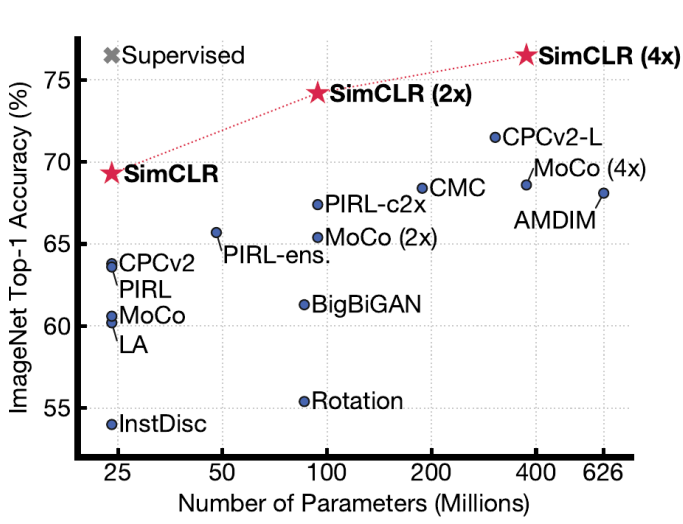
\includegraphics[width=0.6\textwidth]{Images/Chapter2/simclr-results.png}
\caption{دقت روش \lr{SimCLR}}
\label{fig:simclr-results}
\end{figure}
در این معادله،
$1_{[k \neq i]}\in\{0,1\}$
بیانگر تابع نشانگر\LTRfootnote{Indicator function}
می‌باشد که برای تمامی $k$ها
نابرابر با $i$
برابر با یک می‌باشد.
پارامتر $\tau$
تمرکز توزیع را کنترل می‌کند. هر چه
$\tau$
کوچک‌تر، شیب‌ها تیزتر
تابع $sim$
نیز بیانگر یک معیار سنجش شباهت بین نمونه‌ها می‌باشد. در مقاله اصلی از تابع
شباهت کسینوسی\LTRfootnote{Cosine Similarity}
استفاده شده که فرمول آن به فرم معادله
\ref{eq:simclr-cosine} می‌باشد.
شباهت کسینوسی بیانگر کسینوس زاویه‌ی بین دو بردار می‌باشد. هر چه دو بردار در یک جهت باشند، کسینوس زاویه‌ی بین آن‌ها بیشینه و به یک نزدیک می‌شود و هر چه در خلاف جهت یکدیگر باشند، کسینوس زاویه‌ی بین آن‌ها کمینه و به  منفی یک نزدیک می‌شود. بنابراین این تابع هزینه
$f_\theta$ و به تبع آن $g_\phi$
را وادار می‌کند که نگاشت مربوط به نمونه‌های مثبت در یک جهت قرار گیرند و تا جای ممکن در جهت مخالف نسبت به دیگر نمونه‌های دسته باشند.

تابع هزینه استفاده شده در معادله \ref{eq:simclr-loss}،
آنتروپی متقاطع نرمال‌شده با مقیاس دمایی
(\lr{NT-Xent}\LTRfootnote{Normalized Temperature-scaled Cross-Entropy loss}) است که فرمی از تابع \lr{InfoNCE}
می‌باشد. می‌توان نشان داد که با افزایش تعداد منفی‌ها و کمینه کردن این هزینه، کران پایین روی
اطلاعات متقابل\LTRfootnote{Mutual Information}
بین نماها افزایش می‌یابد. یعنی این که با کمینه کردن این تابع هزینه هنگامی که از تعداد نمونه‌های زیادی در یک دسته استفاده کرده‌ایم، مدل یاد می‌گیرد که اطلاعات متقابل بین نمونه‌های مثبت را افزایش دهد و در واقع بازنمایی‌های پایدارتر و کاربردی‌تری را از روی داده‌ها بیاموزد.
\begin{table}[t]
\centering
\caption{دقت روش \lr{SimCLR} در یادگیری انتقالی}
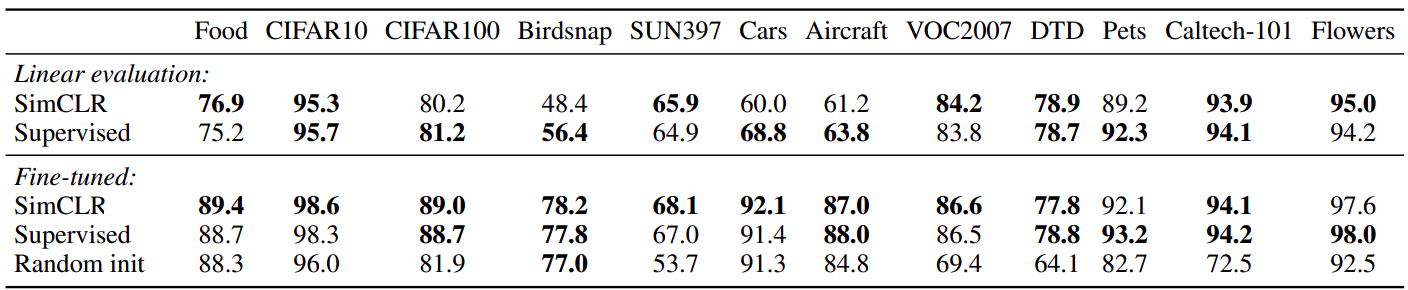
\includegraphics[width=1\textwidth]{Images/Chapter2/simclr-transfer.png}
\label{tab:simclr-transfer}
\end{table}
در نهایت پس از پایان پیش‌آموزش مدل، شبکه‌ی نگاشت به‌کل کنار گذاشته می‌شود چرا که برای وظیفه‌ی یادگیری تباینی و هزینه‌ی \lr{NT-Xent}
آموزش دیده بود. سپس یک شبکه‌ی تماما متصل دیگر به‌عنوان یک دسته‌بند به‌جای شبکه‌ی نگاشت قرار داده می‌شود و یادگیری را بر روی مجموعه داده برچسب‌دار انجام می‌دهیم.

همانطور که در شکل \ref{fig:simclr-results}
می‌توان دید، با افزایش پارامترها دقت روش \lr{SimCLR}
بهبود بسیاری یافته؛ تا جایی که به دقت روش نظارت‌شده رسیده و قابل مقایسه با آن شده است. اما نکته‌ی بسیار مهم روش \lr{SimCLR}
قابلیت تعمیم‌پذیری آن است. همانطور که در جدول \ref{tab:simclr-transfer}
می‌توان دید، عملکرد روش \lr{SimCLR}
در یادگیری انتقالی با روش‌های نظارت‌شده برابری می‌کند و در بسیاری از موارد از آن‌ها پیشی گرفته است.

\subsubsection{پردازش زبان طبیعی}
پردازش زبان طبیعی\LTRfootnote{Natural Language Processing - NLP} یکی از مهم‌ترین شاخه‌های هوش مصنوعی است که هدف آن تعامل مؤثر میان انسان و ماشین از طریق زبان طبیعی می‌باشد. در سال‌های اخیر، یادگیری خودنظارتی پیشرفت‌های شگرفی را در این حوزه رقم زده است. این رویکرد با بهره‌گیری از حجم عظیمی از داده‌های بدون برچسب و تعریف وظایف پیش‌بینی کمکی (مانند پیش‌بینی واژه‌های حذف‌شده یا پیش‌بینی جمله‌ی بعدی) و همچنین با بهره‌گیری از مدل مبدل\LTRfootnote{Transformer}\cite{vaswani2017attention}، امکان یادگیری نمایش‌های زبانی قدرتمند و غنی را فراهم ساخته است. مزیت اصلی این روش در مقایسه با یادگیری نظارت‌شده، عدم نیاز به برچسب‌گذاری دستی داده‌ها و قابلیت تعمیم بهتر مدل به وظایف گوناگون زبان طبیعی است. ظهور مدل‌هایی همچون \lr{BERT\LTRfootnote{Bidirectional Encoder Representations from Transformers}} و \lr{GPT\LTRfootnote{Generative Pre-Trained Transformer}}، که بر مبنای یادگیری خودنظارتی آموزش دیده‌اند، باعث ایجاد جهشی چشمگیر در کیفیت حل مسائل متنوع پردازش زبان طبیعی مانند ترجمه ماشینی، درک مطلب، و تولید متن شده است. علاوه بر این، استفاده از تمام داده‌های متنی موجود در آموزش، این امکان را فراهم می‌کند که اندازه و ظرفیت مدل (تعداد پارامترها) را به‌طور قابل‌توجهی افزایش دهیم، بی‌آن‌که به‌سادگی دچار بیش‌برازش شویم. این رویکرد منجر به پیدایش نسل جدیدی از مدل‌ها شده که با نام مدل‌های زبانی بزرگ (\lr{LLM\LTRfootnote{Large Language Models}}) شناخته می‌شوند و قادرند طیف گسترده‌ای از وظایف زبانی را تنها با یک فرایند آموزش عمومی، بدون نیاز به بازآموزی ویژه، انجام دهند. در ادامه، دو مدل \lr{BERT} و \lr{GPT} به‌عنوان نمونه‌های شاخص این رویکرد مورد بررسی قرار می‌گیرند.\newline

\noindent\textbf{مدل \lr{BERT}}

مدل \lr{BERT} که توسط \lr{Devlin} و همکاران\cite{devlin2019bert} معرفی شد،
یک معماری بر مدل مبدل است که با هدف یادگیری بازنمایی‌های زبانی عمیق و دوسویه طراحی شده است. بر خلاف مدل‌های پیشین که جهت پردازش را محدود به چپ‌به‌راست یا راست‌به‌چپ می‌کردند،
\lr{BERT}
از خودتوجهی دوسویه\LTRfootnote{Bidirectional Self-attention}
بهره می‌گیرد و در هر لایه به تمام کلمات موجود در جمله، هم از سمت چپ و هم از سمت راست، توجه می‌کند. این ویژگی باعث می‌شود که مدل بتواند وابستگی‌های معنایی پیچیده را به‌شکل دقیق‌تری مدل‌سازی کند.

مدل \lr{BERT} با استفاده از دو وظیفه‌ی پوششی آموزش داده می‌شود:
\begin{enumerate}
    \item \textbf{وظیفه مدل‌سازی زبان پوشیده\LTRfootnote{Masked Language Modeling}:}
    در این روش، درصدی از توکن‌های ورودی به‌صورت تصادفی با یک نشانه ویژه جایگزین می‌شوند و مدل باید با استفاده از بافت دوطرفه، توکن‌های پوشیده را پیش‌بینی کند. این کار باعث می‌شود که مدل به‌طور همزمان از اطلاعات گذشته و آینده در جمله بهره ببرد.
    \item \textbf{وظیفه پیش‌بینی جمله بعدی:}
    در این وظیفه، به مدل دو جمله ارائه می‌شود و مدل باید تشخیص دهد که آیا جمله دوم واقعا در متن اصلی پس از جمله اول آمده یا خیر. این مرحله به \lr{BERT} کمک می‌کند تا روابط سطح جمله و انسجام متنی را بیاموزد.
\end{enumerate}
پس از پیش‌آموزش، \lr{BERT} می‌تواند برای طیف وسیعی از وظایف زبانی مانند دسته‌بندی متون، پاسخ به پرسش، برچسب‌گذاری توالی و استنتاج معنایی تنظیم دقیق شود.\newline

\noindent\textbf{مدل \lr{GPT}}

مدل‌های \lr{GPT}\cite{radford2019language} که توسط \lr{OpenAI} معرفی شدند، همانند مدل \lr{BERT}
بر پایه معماری مبدل ساخته شده‌اند. اما برخلاف \lr{BERT}
که از کدگذار مدل مبدل استفاده می‌کند، مدل \lr{GPT}
فقط از رمزگشای مدل مبدل استفاده می‌کند. ایده‌ی اصلی \lr{GPT}
این است که:
\begin{enumerate}
    \item یک مدل زبانی بزرگ و قدرتمند را به صورت پیش‌آموزش روی یک مجموعه‌داده بسیار عظیم و بدون برچسب، با هدف پیش‌بینی کلمه بعدی آموزش دهد.
    \item مدل پیش‌آموزش یافته را با تنظیم دقیق روی داده‌های برچسب‌دار برای وظایف خاص مانند پرسش و پاسخ تطبیق دهد.
\end{enumerate}
نحوه آموزش \lr{GPT} به فرم مدل‌سازی زبانی خودهمبسته است. یعنی احتمال یک توالی
$(x_1, x_2, \dots, x)$
را به شکل معادله زیر مدل می‌کند:
\begin{equation}
P(x_1, x_2, \dots, x_T) = \prod_{t=1}^{T} P(x_t | x_1, \dots, x_{t-1})
\end{equation}
بنابراین مدل در طول آموزش، سعی دارد که کلمات بعدی متن ورودی را صرفا با دانستن کلمات قبلی پیش‌بینی کند.

سپس مدل بر روی مجموعه داده برچسب‌دار تنظیم دقیق می‌شود و از آن برای وظایفی مانند پرسش و پاسخ استفاده می‌شود.

\section{شناسایی فعالیت انسان با استفاده از یادگیری خودنظارتی}

در فصل حاضر، ابتدا روش‌ها و رویکردهای متداول در حوزه‌ی شناسایی فعالیت انسان با استفاده از داده‌های حسگر بررسی شد و سپس یادگیری خودنظارتی به عنوان یکی از رویکردهای نوین یادگیری ماشین که بدون نیاز به داده‌های برچسب‌خورده قادر به استخراج ویژگی‌های معنادار است، معرفی گردید. ترکیب این دو حوزه، یعنی به‌کارگیری یادگیری خودنظارتی در مسئله‌ی شناسایی فعالیت انسان، به دلیل پتانسیل بالای آن در کاهش وابستگی به داده‌های برچسب‌خورده و استفاده‌ی موثر از داده‌های خام، در سال‌های اخیر مورد توجه گسترده‌ی پژوهشگران قرار گرفته است.

با توجه به این که فرایند برچسب‌گذاری داده‌های حسگر، به‌ویژه در سناریوهای واقعی و مقیاس بزرگ، زمان‌بر، پرهزینه و مستعد خطا است، وجود رویکردهایی که بتوانند از داده‌های بدون برچسب بهره‌برداری کنند، اهمیت بالایی دارد. علاوه بر آن، چالش‌های دیگری نیز برای مسئله‌ی شناسایی فعالیت وجود دارند که به‌طور خلاصه شامل موارد زیر می‌باشد:
\begin{enumerate}
    \item وقتی که کاربران مختلف یک فعالیت را انجام می‌دهند، به‌دلیل تفاوت‌هایی که در فیزیولوژی افراد وجود دارد، ممکن است که برای یک فعالیت مشابه داده‌های دارای توزیع‌های نسبتا متفاوت تولید شود.
    \item حرکت کاربر در طول زمان بسته به مواردی مانند خستگی ممکن است تغییر کند.
    \item ویژگی‌های مربوط به سالمندان و جوانان متفاوت هستند.
    \item در استفاده‌ی عملی از شناسایی فعالیت توسط یادگیری عمیق با تعداد زیادی کاربران جدید مواجه خواهیم شد.
\end{enumerate}
یادگیری خودنظارتی با تعریف وظایف کمکی و استفاده از ساختار ذاتی داده‌ها، این امکان را فراهم می‌سازد که بازنمایی‌های غنی و تعمیم‌پذیری از داده‌های خام به‌دست آید، که در ادامه می‌توان آن‌ها را در مدل‌های نظارت‌شده برای شناسایی فعالیت انسان به‌کار گرفت. از سوی دیگر، حجم بسیار بالای داده‌های خام حسگر که از دستگاه‌هایی نظیر تلفن‌های همراه، ساعت‌های هوشمند، مچ‌بندهای سلامتی و سامانه‌های سنجش محیطی به دست می‌آید، فرصت کم‌نظیری برای بهره‌گیری از این رویکرد فراهم می‌کند. با این حال، به‌کارگیری یادگیری خودنظارتی در حوزه‌ی شناسایی فعالیت انسان با چالش‌هایی نیز همراه است؛ از جمله طراحی وظایف کمکی مناسب برای داده‌های زمانی چندحسگری و استفاده از روش‌های مناسب برای داده‌افزایی.

در ادامه به بررسی پژوهش‌های انجام شده در زمینه‌ی شناسایی فعالیت با استفاده از یادگیری خودنظارتی می‌پردازیم.

\subsection{سابقه پژوهش}

در حوزه‌ی شناسایی فعالیت انسان با استفاده از یادگیری خودنظارتی کارهای متعددی انجام شده است. در این بخش به بررسی تعدادی از روش‌های موفقیت‌آمیز در این حوزه می‌پردازیم.

\subsubsection{شناسایی فعالیت مبتنی بر روش \lr{CPC}}

با تکیه بر توضیحاتی که پیش‌تر در بخش \ref{sec:CPC} درباره‌ی روش \lr{CPC}\cite{oord2018representation} ارائه شد، در اینجا نحوه‌ی استفاده از آن در شناسایی فعالیت انسان بررسی می‌شود. \lr{Haresamudram} و همکاران\cite{haresamudram2021contrastive} از روش \lr{CPC} برای ایجاد بازنمایی ویژگی از داده‌های حسگر بهره برده‌اند. در این مطالعه، داده‌های خام حسگرها به قطعات زمانی هم‌پوشان تقسیم می‌شوند. سپس یک شبکه‌ی کدگذار مبتنی بر شبکه‌های پیچشی، بازنمایی‌های سطح بالا را برای هر قطعه استخراج می‌کند. پس از آن، همانند روش \lr{CPC}، از یک مدل مبتنی بر \lr{GRU} به‌عنوان کدگذار خودهمبسته استفاده شده و هزینه‌ی تباینی بر روی پیش‌بینی بازنمایی‌ها اعمال می‌شود.

\begin{table}[htbp]
\centering
\caption{نتایج روش \lr{CPC} در شناسایی فعالیت}
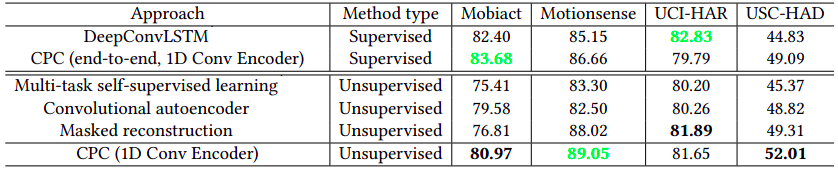
\includegraphics[width=1\textwidth]{Images/Chapter2/har-cpc-results.png}
\label{tab:har-cpc-results}
\end{table}

پس از اتمام مرحله‌ی پیش‌آموزش، کدگذار آموزش‌دیده با وزن‌های تثبیت‌شده برای استخراج ویژگی به یک مدل دسته‌بندی کاملاً متصل منتقل می‌شود تا آموزش نظارت‌شده انجام شود. همان‌طور که در جدول \ref{tab:har-cpc-results} مشاهده می‌شود، عملکرد این روش در بیشتر معیارها قابل قبول است و در برخی موارد حتی از مدل‌های کاملاً نظارت‌شده پیشی گرفته است.

\subsubsection{شناسایی فعالیت مبتنی بر روش \lr{SimCLR}}

روش \lr{SimCLR}\cite{chen2020simple} که پیش‌تر در بخش \ref{sec:simclr} معرفی شد، یکی از چارچوب‌های مطرح در یادگیری خودنظارتی مبتنی بر یادگیری تباینی است؛ اما این روش در اصل برای داده‌های تصویری ارائه شده و برای استفاده بر روی داده‌های حسگر نیازمند تغییرات و انطباق‌هایی است.

خارتدینف و همکاران\cite{khaertdinov2021contrastive} چارچوبی با عنوان \lr{CSSHAR}\LTRfootnote{Contrastive Self-Supervised Human Activity Recognition} ارائه دادند که نسخه‌ی سازگارشده‌ی \lr{SimCLR} برای شناسایی فعالیت انسان با داده‌های حسگر است. در این رویکرد، به‌جای شبکه‌های پیچشی، از یک معماری مبتنی بر مبدل (\lr{Transformer}) برای استخراج ویژگی استفاده شده است. همچنین به دلیل ماهیت متفاوت سیگنال‌های زمانی نسبت به تصاویر، مجموعه‌ای از داده‌افزایی‌های اختصاصی برای حسگرها طراحی شده که شامل موارد زیر است:

\begin{itemize}
\item \textbf{افزودن نویز:} اضافه‌کردن نویز گوسی تصادفی به سیگنال.
\item \textbf{مقیاس‌گذاری\LTRfootnote{Scaling}:} ضرب دامنه‌ی سیگنال در ضریب تصادفی از یک توزیع گوسی.
\item \textbf{چرخاندن:} معکوس‌کردن علامت نمونه‌های انتخاب‌شده به‌صورت تصادفی.
\item \textbf{جایگشت\LTRfootnote{Permutation}:} تقسیم سیگنال به چند بخش و جابه‌جایی تصادفی مقادیر در این بخش‌ها.
\end{itemize}

بسته به ویژگی‌های مجموعه‌داده، ممکن است همه یا تنها تعدادی از این تبدیلات به‌کار گرفته شوند که این انتخاب به‌صورت تجربی و با آزمون و خطا انجام می‌شود. پس از ایجاد نماهای مختلف از هر نمونه، آن‌ها به یک شبکه‌ی نگاشت (\lr{Projection Head}) وارد می‌شوند و تابع هزینه‌ی تباینی \lr{NT-Xent} برای یادگیری بازنمایی‌ها به‌کار می‌رود. در مرحله‌ی تنظیم دقیق، شبکه‌ی نگاشت حذف‌شده و یک دسته‌بند کاملاً متصل جایگزین آن می‌گردد. در این مرحله، وزن‌های کدگذار مبتنی بر مبدل ثابت نگه داشته می‌شوند تا سرعت آموزش افزایش یابد.

\begin{table}[htbp]
\centering
\caption{نتایج روش \lr{CSSHAR}}
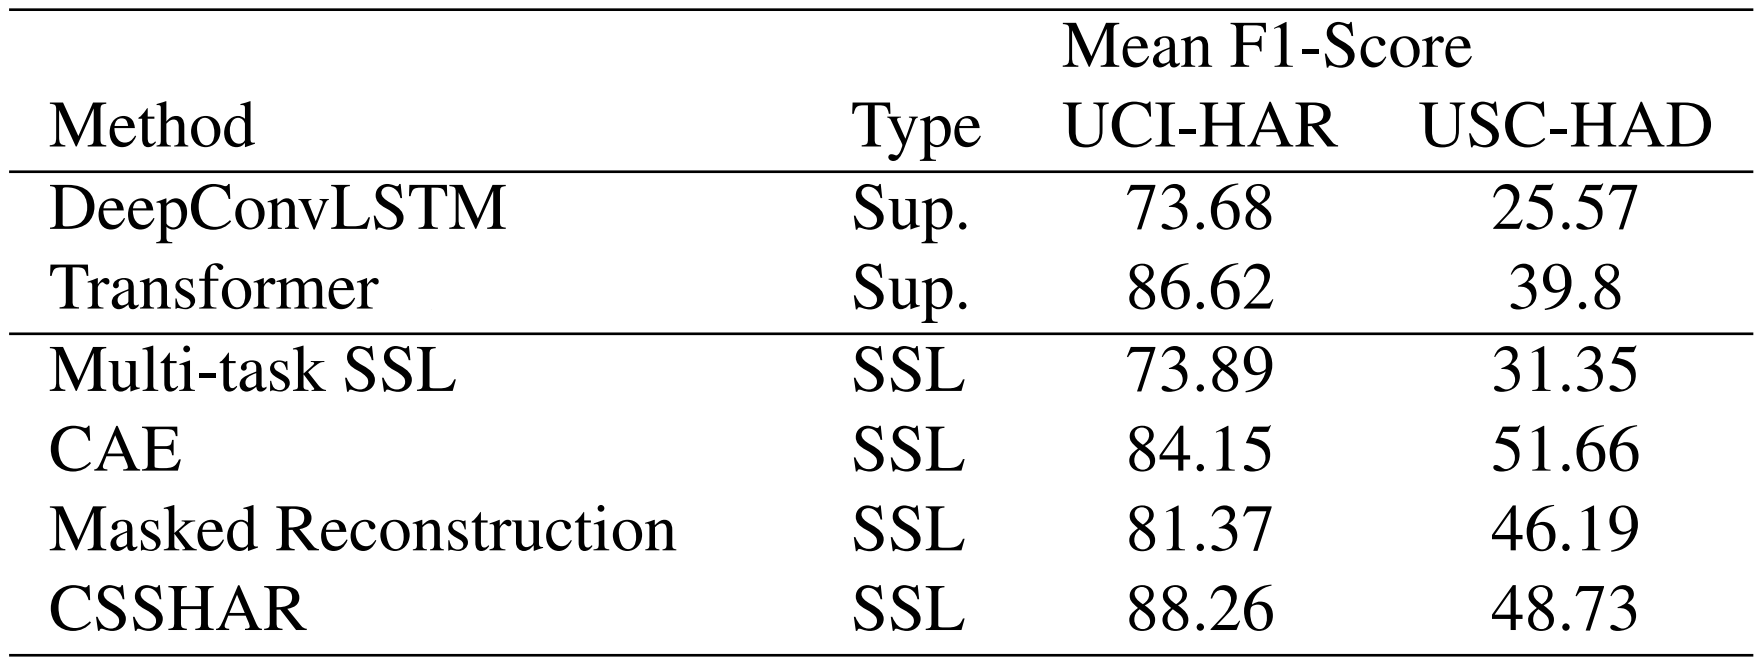
\includegraphics[width=0.75\textwidth]{Images/Chapter2/csshar-results.png}
\label{tab:csshar-results}
\end{table}

همان‌طور که در جدول \ref{tab:csshar-results} مشاهده می‌شود، ترکیب سازوکار یادگیری تباینی \lr{SimCLR} با توانایی مبدل در مدل‌سازی وابستگی‌های طولانی‌مدت سیگنال، به بهبود قابل‌توجه دقت در شناسایی فعالیت منجر شده است. این روش به‌ویژه در شرایطی که داده‌های برچسب‌خورده محدود هستند، عملکردی رقابتی یا حتی برتر نسبت به مدل‌های نظارت‌شده نشان داده است.

\subsubsection{شناسایی فعالیت مبتنی بر یادگیری مشارکتی}

جین و همکاران \cite{jain2022collossl} یک چارچوب یادگیری خودنظارتی نوین و مشارکتی\LTRfootnote{Collaborative} تحت عنوان \lr{ColloSSL} را برای پیش‌آموزش مدل‌های بازشناسی فعالیت انسان ارائه دادند. این روش برای محیط‌هایی طراحی شده است که در آن چندین حسگر به‌طور همزمان داده‌های مربوط به یک فعالیت را ثبت می‌کنند. این محیط، یک سیستم چند دستگاهی همگام با زمان (\lr{TSMDS}\LTRfootnote{Time-Synchronous Multi-Device System}) نامیده می‌شود که در آن، داده‌های ثبت‌شده توسط حسگرهای مختلف کاملا همگام هستند.

ایده‌ی اصلی \lr{ColloSSL} این است که به‌جای تولید داده‌های افزوده به‌صورت مصنوعی (مانند افزودن نویز یا دوران)، از داده‌های حسگرهای مختلف به‌عنوان تبدیل‌های طبیعی \LTRfootnote{Natural Transformations} از یکدیگر استفاده شود. به عبارت دیگر، داده‌ی ثبت‌شده توسط حسگر روی مچ دست و حسگر روی قفسه‌ی سینه، دو «نما» یا «دیدگاه» متفاوت از یک فعالیت یکسان (مثلا راه‌رفتن) هستند. هدف یادگیری تباینی در این روش، نزدیک کردن بازنمایی این نماهای مختلف از یک فعالیت و دورکردن آن‌ها از بازنمایی فعالیت‌های دیگر است.

\begin{figure}[t]
\centering
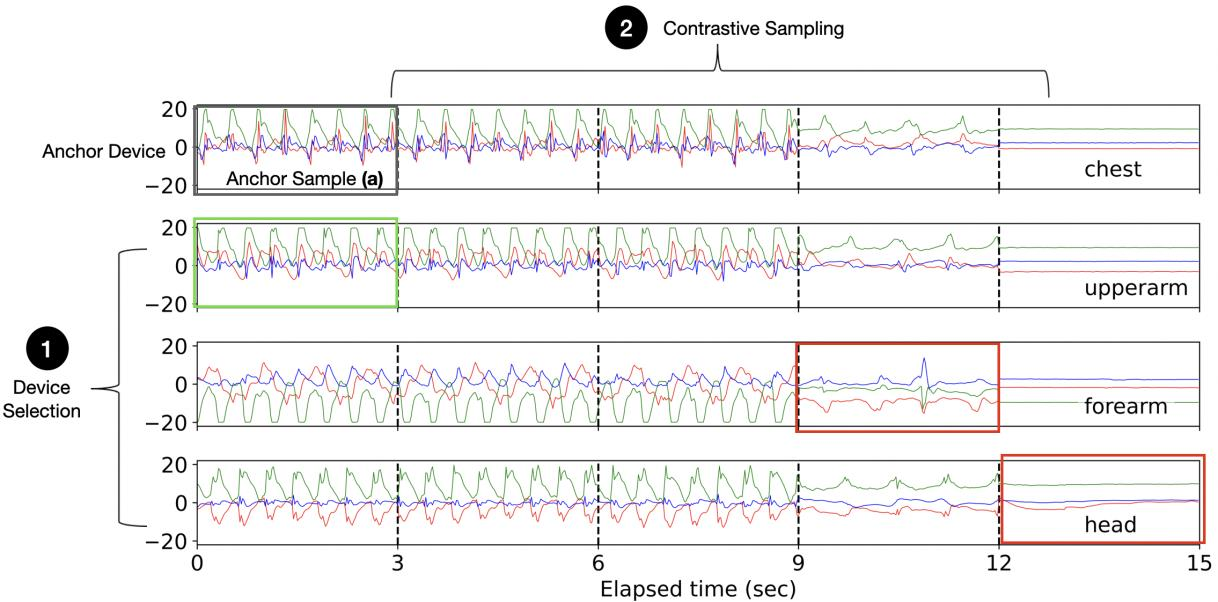
\includegraphics[width=1\textwidth]{Images/Chapter2/collossl.png}
\caption{انتخاب حسگرهای مثبت و منفی در \lr{ColloSSL}}

\label{fig:collossl}

\end{figure}

برای مثال، همانطور که در شکل \ref{fig:collossl} نمایش داده شده است، فرض کنید می‌خواهیم مدل را با محوریت داده‌های حسگر قفسه سینه پیش‌آموزش دهیم. در این حالت، این حسگر به‌عنوان دستگاه محوری \LTRfootnote{Anchor Device} انتخاب می‌شود. سپس، نمونه‌های داده از این دستگاه با نمونه‌های سایر دستگاه‌ها مقایسه می‌شوند. فرایند کلی یادگیری در این مقاله به‌صورت زیر است:

\begin{enumerate}
\item ابتدا، یک استخراج‌کننده‌ی ویژگی (در این مقاله، یک شبکه‌ی پیچشی یک‌بعدی با سه لایه) با وزن‌های تصادفی مقداردهی اولیه می‌شود.
\item یک دسته‌ی تصادفی از داده‌ها انتخاب می‌شود. این دسته شامل پنجره‌های زمانی (مثلا به طول ۳ ثانیه) از تمام حسگرها است. نکته‌ی کلیدی این است که این پنجره‌ها از نظر زمانی با یکدیگر همگام هستند.
\item برای شروع یادگیری تباینی، یک نمونه از یک دستگاه خاص (مثلاً قفسه سینه) به‌عنوان نمونه‌ی محوری \LTRfootnote{Anchor Sample} انتخاب می‌شود.
\item نمونه‌های زمانی متناظر با نمونه‌ی محوری از سایر دستگاه‌ها (مانند مچ، ران و غیره) به‌عنوان نمونه‌های مثبت در نظر گرفته می‌شوند. این نمونه‌ها دیدگاه‌های متفاوتی از همان فعالیت در همان لحظه هستند.
\item تمام نمونه‌های دیگر در آن دسته (که متعلق به پنجره‌های زمانی دیگری هستند) به‌عنوان نمونه‌های منفی انتخاب می‌شوند.
\item تمام این نمونه‌ها (محوری، مثبت و منفی) به استخراج‌کننده‌ی ویژگی داده می‌شوند تا بازنمایی نهفته‌ی آن‌ها استخراج شود. سپس با استفاده از یک تابع زیان تباینی، مدل آموزش داده می‌شود. هدف این تابع زیان، به حداکثر رساندن شباهت بین بازنمایی نمونه‌ی محوری و نمونه‌های مثبت، و به حداقل رساندن شباهت آن با نمونه‌های منفی است.
\item مراحل ۳ تا ۶ برای تمام نمونه‌های موجود در دسته تکرار می‌شوند تا مدل به‌طور کامل یاد بگیرد که چگونه بازنمایی‌های معناداری از فعالیت‌ها استخراج کند. این فرایند با انتخاب دسته‌های جدید ادامه می‌یابد.
\end{enumerate}

در نهایت، مزیت کلیدی چارچوب \lr{ColloSSL} در تعریف هوشمندانه‌ی وظیفه‌ی پیش‌آموزشی آن نهفته است. این روش با بهره‌گیری از داده‌های همگامِ حسگرهای مختلف، یک سیگنال نظارتی غنی و طبیعی را بدون نیاز به هیچ‌گونه برچسب‌گذاری انسانی یا افزونه‌سازی مصنوعی ایجاد می‌کند. در نتیجه، استخراج‌کننده‌ی ویژگی حاصل، بازنمایی‌هایی عمیق و پایدار از فعالیت‌های انسانی را فرا می‌گیرد که می‌تواند به‌عنوان یک پایه‌ی قدرتمند برای بهبود عملکرد و کاهش نیاز به داده‌های برچسب‌دار در مدل‌های دسته‌بندی نهایی عمل کند.

\subsubsection{شناسایی فعالیت مبتنی بر یادگیری خودنظارتی چندوظیفه‌ای در مقیاس بزرگ}

مقاله اخیر یوان و همکاران \cite{yuan2024self} یکی از جامع‌ترین و مقیاس‌پذیرترین کارها در زمینه یادگیری خودنظارتی برای شناسایی فعالیت انسان است. هسته مرکزی این پژوهش، استفاده از یک مجموعه داده شدیدا حجیم و بدون برچسب از مطالعه \lr{UK Biobank} متشکل از ۰۰۰,۷۰۰ روز-نفر داده (۰۰۰,۱۰۰ نفر به مدت ۷ روز) شتاب‌سنج مچ دست است.

این پژوهش با الهام از موفقیت‌های یادگیری خودنظارتی در بینایی کامپیوتر و پردازش زبان طبیعی، از یک چارچوب یادگیری خودنظارتی چندوظیفه‌ای \LTRfootnote{Multi-task Self-Supervised Learning} برای پیش‌آموزش یک مدل پایه استفاده می‌کند. این مدل پایه سپس روی هشت مجموعه داده معیار مختلف برای وظیفه اصلی شناسایی فعالیت، تنظیم دقیق شده است.

\noindent\textbf{وظایف خودنظارتی:} سه وظیفه خودنظارتی ساده اما مؤثر برای پیش‌آموزش به کار گرفته شده‌اند که بر درک دینامیک حرکت انسانی تمرکز دارند:
\begin{itemize}
\item \textbf{پیکان زمان\LTRfootnote{Arrow of Time (AoT)}:} در این وظیفه، مدل باید تشخیص دهد که آیا یک سیگنال در جهت طبیعی زمان است یا در خلاف زمان (معکوس) پخش می‌شود. این کار مدل را وادار به یادگیری ویژگی‌های وابسته به جهت زمان می‌کند.
\item \textbf{جایگشت\LTRfootnote{Permutation}:} سیگنال به چند قطعه تقسیم و سپس به صورت تصادفی جابه‌جا می‌شود. مدل باید تشخیص دهد که آیا توالی سیگنال دست‌نخورده است یا قطعات آن جابه‌جا شده‌اند. این کار به مدل در یادگیری وابستگی‌های زمانی کوتاه‌برد کمک می‌کند.
\item \textbf{تغییر شکل زمان\LTRfootnote{Time Warping (TW)}:} بخش‌هایی از سیگنال به صورت تصادفی کشیده یا فشرده می‌شوند تا سرعت حرکت را تغییر دهند. مدل باید این اعوجاج‌های زمانی را تشخیص دهد که منجر به یادگیری ویژگی‌های مستقل از سرعت اجرای فعالیت می‌شود.
\end{itemize}

\noindent\textbf{معماری و آموزش:} نویسندگان از یک شبکه \lr{ResNet} به عنوان استخراج‌کننده ویژگی اصلی استفاده کردند. این شبکه به طور همزمان روی سه وظیفه فوق پیش‌آموزش دید. یک نکته فنی مهم که به پایداری آموزش کمک شایانی کرد، استفاده از نمونه‌برداری وزن‌دار بود. در این روش، به پنجره‌های داده با حرکت بیشتر (انحراف معیار بالاتر) وزن بیشتری داده می‌شود، زیرا پنجره‌های کم‌حرکت (مانند حالت سکون) پس از اعمال تبدیل‌های خودنظارتی تقریباً بدون تغییر می‌مانند و برای آموزش بی‌فایده هستند.

مدل نهایی به طور قابل توجهی و در تمامی هشت مجموعه داده معیار، از شبکه \lr{ResNet} بدون پیش‌آموزش خودنظارتی عملکرد بهتری از خود نشان داد. مهم‌تر از همه، این مدل توانایی تعمیم‌پذیری فوق‌العاده‌ای را در شرایط مختلف از جمله جمعیت‌های مختلف (سالمند، بیماران پارکینسون)، محیط‌های مختلف (آزاد، آزمایشگاهی) و دستگاه‌های مختلف  (برندهای مختلف حسگر) نشان داد. این پژوهش به وضوح نشان می‌دهد که مقیاس داده (حجم و تنوع) در کنار طراحی مناسب وظایف خودنظارتی می‌تواند منجر به ایجاد مدل‌های پایه‌ای شود که مشکل تعمیم‌پذیری را در شناسایی فعالیت انسان به میزان زیادی مرتفع می‌سازند.

\subsubsection{شناسایی فعالیت متقابل-داده‌ای با پیش‌آموزش سلسله‌مراتبی خودنظارتی}

مقاله‌ی «\lr{CrossHAR}» اثر \lr{Hong} و همکاران \cite{hong2024crosshar} به مسئله‌ی مهم شناسایی فعالیت متقابل-داده‌ای (\lr{Cross-Dataset HAR}) می‌پردازد. در این سناریو، مدل تنها با داده‌های یک مجموعه‌داده‌ی منبع آموزش می‌بیند و سپس بر روی مجموعه‌داده‌ی هدف کاملاً جدید و نادیده ارزیابی می‌شود. این چالش به دلیل وجود «تغییر حوزه» (\lr{Domain Shift}) ناشی از تفاوت در کاربران، نوع دستگاه‌ها، مکان قرارگیری حسگرها و پروتکل‌های جمع‌آوری داده بین مجموعه‌داده‌ها، بسیار دشوارتر از حالت متقابل-حوزه‌ای (\lr{Cross-Domain}) درون یک مجموعه‌داده است.

\lr{CrossHAR} یک چارچوب سه‌بخشی برای یادگیری بازنمایی‌های تعمیم‌پذیر ارائه می‌دهد:

\begin{enumerate}
\item \textbf{افزوده‌سازی داده‌ی حسگر مبتنی بر فیزیک (\lr{Physically-informed Sensor Data Augmentation}):} این مؤلفه با الهام از اصول فیزیکی تولید داده‌های \lr{IMU} (شتاب‌سنج و ژیروسکوپ)، به شبیه‌سازی تغییرات در جهت‌گیری دستگاه (\lr{Device Orientation}) می‌پردازد. با اعمال ماتریس تبدیل‌های چرخشی متعامد بر روی کانال‌های داده، داده‌های منبع را به شش جهت مختلف گسترش می‌دهد. این کار باعث افزایش تنوع داده‌ها و کمک به مدل برای یادگیری ویژگی‌های نامتغیر نسبت به چرخش دستگاه می‌شود.
\item \textbf{پیش‌آموزش سلسله‌مراتبی داده‌ی حسگر (\lr{Hierarchical Sensor Data Pretraining}):} این بخش هسته‌ی اصلی یادگیری خودنظارتی در \lr{CrossHAR} است و از دو مرحله تشکیل شده است:
\begin{itemize}
    \item \textbf{مدل‌سازی حسگر پوشیده (\lr{Masked Sensor Modeling}):} با الهام از \lr{BERT} در پردازش زبان، بخش‌هایی از داده‌ی حسگر پوشانده شده و مدل وظیفه بازسازی آن‌ها را بر عهده می‌گیرد. این کار به مدل در یادگیری الگوهای محلی و وابستگی‌های زمانی در داده‌های \lr{IMU} کمک می‌کند.
    \item \textbf{تنظیم‌کردن تباینی (\lr{Contrastive Regularization}):} برای تکمیل مرحله قبل و یادگیری الگوهای سراسری (\lr{Global Patterns})، یک تابع هزینه تباینی نیز به کار گرفته می‌شود. در اینجا، با ایجاد دو «نما» (\lr{View}) از یک نمونه (از طریق تبدیل‌هایی مانند مقیاس‌گذاری و جابه‌جایی بخش‌ها)، مدل یاد می‌گیرد که بازنمایی‌های نمونه‌های مثبت (نماهای مختلف از یک نمونه) را به هم نزدیک و از نمونه‌های منفی (نمونه‌های دیگر) دور کند.
\end{itemize}
نکته کلیدی در اینجا، استفاده از یک پارادایم آموزش ترتیبی است: ابتدا مدل تنها با تابع هزینه بازسازی (\lr{$\mathcal{L}_m$}) آموزش می‌بیند و سپس هر دو تابع هزینه (\lr{$\mathcal{L}_m$} و \lr{$\mathcal{L}_r$}) با هم به روزرسانی می‌شوند. این کار به همگرایی بهتر مدل کمک می‌کند.
\item \textbf{تنظیم دقیق برای شناسایی فعالیت (\lr{Fine-Tune Activity Recognition}):} پس از اتمام پیش‌آموزش خودنظارتی بر روی داده‌های بدون برچسب منبع، مدل پیش‌آموزش‌دیده با استفاده از یک مجموعه کوچک از داده‌های برچسب‌دار منبع، برای کاربرد نهایی شناسایی فعالیت، به‌صورت نظارت‌شده تنظیم دقیق (\lr{Fine-tune}) می‌شود.
\end{enumerate}

نتایج گسترده‌ی آزمایش‌ها بر روی چهار مجموعه‌داده واقعی نشان می‌دهد که \lr{CrossHAR} با اختلاف دقت متوسط \%۱۰.۸۳، از روش‌های مطرح در شناسایی متقابل-داده‌ای پیشی می‌گیرد. همچنین، یک مطالعه موردی با استقرار مدل بر روی یک گوشی هوشمند، کارایی عملی آن را با سرعت استنتاج قابل قبول (۰۲۲۵.۰ ثانیه بر نمونه) نشان می‌دهد.

مزیت اصلی \lr{CrossHAR} در ترکیب هوشمندانه‌ی \textbf{افزوده‌سازی مبتنی بر فیزیک} برای مقابله با تغییر حوزه، و یک \textbf{الگوی پیش‌آموزش سلسله‌مراتبی} برای یادگیری همزمان الگوهای محلی و سراسری از داده‌های حجیم بدون برچسب است. این رویکرد، گامی مهم در جهت ایجاد مدل‌های تعمیم‌پذیر و مستقل برای شناسایی فعالیت انسان در دنیای واقعی محسوب می‌شود.

\subsubsection{شناسایی فعالیت مبتنی بر روش \lr{AttCLHAR}}

چن و همکاران\cite{chen2024enhancing} در مقاله‌ی خود با عنوان «بهبود شناسایی فعالیت انسان در خانه‌های هوشمند با یادگیری خودنظارتی و خودتوجهی»، مدلی نوین به نام \lr{AttCLHAR} را معرفی کردند. این مدل بر پایه‌ی چارچوب \lr{SimCLR} بنا شده و با ادغام مکانیزم خودتوجهی و بهینه‌سازی آگاه از تیزی (\lr{Sharpness-Aware Minimization} یا \lr{SAM})، برای شناسایی فعالیت‌های انسانی با استفاده از داده‌های حسگر محیطی در خانه‌های هوشمند طراحی شده است. معماری پیشنهادی شامل یک کدگذار مبتنی بر شبکه‌ی پیچشی یک‌بعدی، شبکه‌ی مبدل و یک لایه خودتوجهی است که به مدل امکان می‌دهد تا علاوه بر یادگیری وابستگی‌های مکانی-زمانی، بر بخش‌های مرتبط دنباله‌ی ورودی تمرکز کند.

در این روش، فرآیند یادگیری در دو مرحله‌ی پیش‌آموزش بدون ناظر و تنظیم دقیق انجام می‌شود. در مرحله‌ی پیش‌آموزش، از تابع زیان \lr{NT-Xent} در یک چارچوب یادگیری تباینی برای یادگیری بازنمایی‌های معنادار از داده‌های بدون برچسب استفاده می‌شود. همچنین، الگوریتم \lr{SAM} با هدف بهبود تعمیم‌پذیری مدل و کاهش حساسیت به نویز، به کار گرفته شده است. در مرحله‌ی تنظیم دقیق، کدگذار از قبل آموزش‌دیده با مقدار کمی داده برچسب‌دار، برای دسته‌بندی فعالیت‌ها fine-tune می‌شود.

نتایج تجربی بر روی مجموعه‌داده‌های \lr{CASAS} شامل \lr{Aruba-1}، \lr{Aruba-2} و \lr{Milan} نشان می‌دهد که مدل \lr{AttCLHAR} در سناریوهای نیمه‌نظارتی و انتقال یادگیری، عملکردی برتر از مدل‌های پایه و سایر روش‌های متداول دارد. این مدل به‌ویژه در شرایطی که داده‌های برچسب‌خورده محدود هستند، توانایی بالایی در استخراج ویژگی‌های موثر از داده‌های حجیم بدون برچسب نشان داده است.

\subsubsection{شناسایی فعالیت مبتنی بر شبکه دوشاخه‌ای یادگیری ویژگی‌های مکانی-زمانی}

ژان و همکاران \cite{zhan2025single} از یک معماری دوشاخه‌ای برای استخراج همزمان ویژگی‌های مکانی-زمانی محلی و وابستگی‌های بلندمدت زمانی استفاده شده است. این مدل شامل دو شاخه‌ی اصلی است: شاخه‌ی \lr{3D-CNN} برای استخراج الگوهای حرکتی محلی و کوتاه‌مدت، و شاخه‌ی مدل‌سازی زمانی مبتنی بر \lr{GRU} برای یادگیری وابستگی‌های بلندمدت. خروجی این دو شاخه در فضای ویژگی ادغام شده و برای دسته‌بندی نهایی فعالیت‌ها به یک لایه‌ی کاملاً متصل وارد می‌شود. این روش با بهره‌گیری از داده‌های شتاب‌سنج تنها و بدون نیاز به ادغام چنددستگاهی، به دقت بالایی در مجموعه‌داده‌ی \lr{WISDM} دست یافته و از روش‌های پایه‌ای مانند \lr{3DCNN}، \lr{LSTM}، \lr{RNN} و \lr{Transformer} پیشی گرفته است. با این حال، چالش اصلی این مدل، پیچیدگی محاسباتی نسبتاً بالای آن است که امکان استقرار روی سامانه‌های نهفته را با محدودیت مواجه می‌سازد.

\section{جمع‌بندی}

در این فصل، ادبیات موضوع و کارهای پیشین در حوزه‌ی شناسایی فعالیت انسان و یادگیری خودنظارتی مورد بررسی قرار گرفت. ابتدا به بررسی روش‌های شناسایی فعالیت انسان پرداختیم. سپس چالش اصلی روش‌های یادگیری عمیق، یعنی نیاز به حجم بالای داده‌های برچسب‌دار، تشریح شد. در ادامه، یادگیری خودنظارتی به‌عنوان یک راهکار موثر برای غلبه بر این محدودیت معرفی گردید که با تعریف وظایف پوششی بر روی داده‌های خام، به یادگیری بازنمایی‌های غنی می‌پردازد. در نهایت، با مرور پژوهش‌های ترکیبی در این دو حوزه، نشان داده شد که اقتباس روش‌های خودنظارتی، به‌ویژه رویکردهای تباینی، برای داده‌های حسگری به نتایج امیدوارکننده‌ای منجر شده و می‌تواند عملکردی قابل مقایسه با روش‌های کاملاً نظارت‌شده، با نیاز به مراتب کمتری به داده‌های برچسب‌دار، ارائه دهد.
